\documentclass{article}
\usepackage{microtype}
\usepackage{graphicx}
\usepackage{subcaption}
\usepackage{booktabs} % for professional tables
\usepackage{hyperref}
\newcommand{\theHalgorithm}{\arabic{algorithm}}
\usepackage[preprint]{icml2026}
\usepackage{amsmath}
\usepackage{amssymb}
\usepackage{mathtools}
\usepackage{amsthm}
\usepackage{comment}
\newcommand{\method}{{\textsc{DiSPO}}}
\usepackage[dvipsnames,table]{xcolor}
\newcommand{\action}[1]{\textbf{\textcolor{JungleGreen}{#1}}}
\newcommand{\state}[1]{\textbf{\textcolor{Orange}{#1}}}
\newcommand{\hlline}[2][yellow!20]{%
  \colorbox{#1}{#2}%
}

\usepackage{tikz}
\usetikzlibrary{tikzmark}
\usepackage[most]{tcolorbox}
\usepackage{url}
\usepackage{multirow} %
\newtcbox{\roundboxgray}[1][gray!18]{
  on line,
  colback=#1,
  colframe=#1,
  boxrule=0pt,
  arc=3pt,
  boxsep=2pt,
  left=0pt, right=0pt, top=0pt, bottom=0pt
}
\newtcbox{\roundboxblue}[1][blue!10]{
  on line,
  colback=#1,
  colframe=#1,
  boxrule=0pt,
  arc=3pt,
  boxsep=1pt,
  left=0pt, right=0pt, top=0pt, bottom=0pt
}
\newtcbox{\roundboxorange}[1][orange!10]{
  on line,
  colback=#1,
  colframe=#1,
  boxrule=0pt,
  arc=3pt,
  boxsep=1pt,
  left=0pt, right=0pt, top=0pt, bottom=0pt
}


%%%%%%%%%%%%%%%%%%%%%%


% if you use cleveref..
\usepackage[capitalize,noabbrev]{cleveref}

%%%%%%%%%%%%%%%%%%%%%%%%%%%%%%%%
% THEOREMS
%%%%%%%%%%%%%%%%%%%%%%%%%%%%%%%%
\theoremstyle{plain}
\newtheorem{theorem}{Theorem}[section]
\newtheorem{proposition}[theorem]{Proposition}
\newtheorem{lemma}[theorem]{Lemma}
\newtheorem{corollary}[theorem]{Corollary}
\theoremstyle{definition}
\newtheorem{definition}[theorem]{Definition}
\newtheorem{assumption}[theorem]{Assumption}
\theoremstyle{remark}
\newtheorem{remark}[theorem]{Remark}
\usepackage[textsize=tiny]{todonotes}

\icmltitlerunning{Diffusion-State Policy Optimization for Masked Diffusion Language Models}

\begin{document}
\twocolumn[
\icmltitle{Diffusion-State Policy Optimization for Masked Diffusion Language Models}
\icmlsetsymbol{equal}{*}

  \begin{icmlauthorlist}
    \icmlauthor{Daisuke Oba}{isct}
    \icmlauthor{Hiroki Furuta}{independent}
    \icmlauthor{Naoaki Okazaki}{isct}
  \end{icmlauthorlist}

  \icmlaffiliation{isct}{Department of Computer Science, Institute of Science Tokyo, Japan}
  \icmlaffiliation{independent}{Tokyo, Japan}
  \icmlcorrespondingauthor{Daisuke Oba}{daisuke.oba@nlp.comp.isct.ac.jp}
  \icmlkeywords{Diffusion Language Models, Reinforcement Learning}
  \vskip 0.3in
]
\printAffiliationsAndNotice{}  % no special notice (required even if empty)

\begin{abstract}
Masked diffusion language models generate by iteratively filling masked tokens over multiple denoising steps, so learning only from a terminal reward on the final completion yields coarse credit assignment over intermediate decisions.
We propose \method\ (Diffusion-State Policy Optimization), a plug-in credit-assignment layer that directly optimizes intermediate filling decisions.
At selected intermediate masked states, \method\ branches by resampling fillings for the currently masked positions from rollout-cached logits, scores the resulting completions, and updates only the newly filled tokens---without additional multi-step diffusion rollouts.
We formalize a fixed-state objective for branched completions and derive a policy-gradient estimator that can be combined with terminal-feedback policy optimization using the same rollouts.
On LLaDA-8B-Instruct, \method\ consistently improves over the terminal-feedback diffu-GRPO baseline on math and planning benchmarks under matched rollout compute and optimizer steps. 
Our code will be available at \url{https://daioba.github.io/dispo}.
\end{abstract}

\begin{figure}[t]
    \centering
    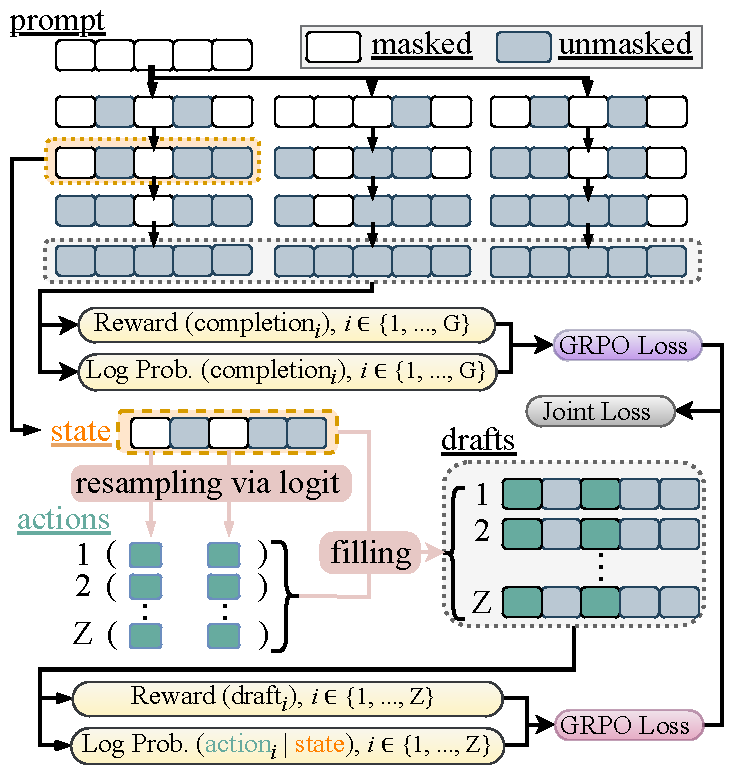
\includegraphics[width=0.43\textwidth]{DiSPO-13.pdf}
    \caption{\textbf{Conceptual overview.}
    \textbf{\emph{Top}}: \emph{Terminal-feedback GRPO} treats the denoising trajectory as one decision.
    \textbf{\emph{Bottom}}: DiSPO is a \emph{plug-in} step that branches at \state{intermediate states} (resample $Z$ fillings from cached logits), scores them with the same reward, and backpropagates gradients only through \action{the filled tokens}.}
    \label{fig:concept}
\end{figure}


\section{Introduction}\label{sec:intro}
Policy optimization (PO) is a standard tool for improving the reasoning and alignment behavior of language models, spanning preference-based RLHF~\citep{ziegler2019fine,stiennon2020summarize,ouyang2022training} and policy-gradient methods~\citep{schulman2015trust,schulman2017proximal}, including recent PPO-style variants for reasoning~\citep{shao2024deepseekmath}.
Most PO setups, however, rely on a scalar reward computed on the final completion and broadcast it uniformly across tokens, which yields coarse credit assignment.

This limitation is especially acute for masked diffusion language models (MDLMs), which generate by repeatedly filling masked positions over multiple denoising steps~\citep{austin2021structured,sahoo2024simple,shi2024simplified,nie2025largelanguagediffusionmodels,ye2025dream,gong2025diffucoder}.
Early fillings constrain what can be fixed later, so success depends on a sequence of intermediate decisions.
Recent work goes beyond purely terminal feedback, e.g., via reward shaping based on intermediate states or trajectory-level comparisons at fixed steps~\citep{sapo,mdpo}.
{{Our key difference is the optimization unit:}} instead of optimizing over denoising trajectories, we optimize state-conditioned mask fillings by holding an intermediate masked sequence fixed and resampling alternative fillings.

To address this gap, we propose \method\ (\emph{Diffusion-State Policy Optimization}; Fig.~\ref{fig:concept}), a plug-in credit-assignment layer that optimizes intermediate filling decisions via fixed-state comparisons (\S~\ref{sec:method}).
Motivated by the policy-gradient formulation~\citep{williams1992simple,sutton1999policy}, we treat a partially-masked sequence as the \state{state} and the token assignments to its masked positions as the \action{action}.
At selected intermediate states, \method\ resamples multiple candidate fillings from rollout-cached logits, forms draft completions, evaluates the same terminal reward, and updates only the newly filled tokens.
Because each denoising step outputs distributions for all masked positions, this branching reuses rollout logits and requires no additional multi-step diffusion rollouts.
\method\ is modular and can be trained jointly with standard terminal-feedback policy optimization (Alg.~\ref{alg:dispo}).

We formalize a fixed-state expected-return objective for intermediate-state branching and show that \method\ yields a valid policy-gradient estimator for it (Theorem~\ref{thm:step-pg}).
Moreover, the step-wise update reuses the same rollouts as terminal-feedback policy optimization (Fig.~\ref{fig:concept}), so the two objectives can be optimized jointly as a single mixed objective in expectation (Theorem~\ref{thm:mixed}).
Finally, restricting updates to newly filled tokens and averaging over same-state branches reduces variance in step-wise gradient (Propositions~\ref{prop:var} and~\ref{prop:compute}).


We evaluate \method\ on LLaDA-8B-Instruct~\citep{nie2025largelanguagediffusionmodels} under the same terminal-feedback training recipe used in prior MDLM policy optimization~\citep{zhao2025d1}.
For a controlled comparison, we match the dominant training costs---multi-step diffusion rollouts and optimizer update steps---so improvements reflect finer state-conditioned credit assignment rather than extra rollouts.
Across math reasoning (GSM8K~\citep{gsm8k} and MATH500~\citep{lightman2023lets}) and symbolic planning (Sudoku and Countdown~\citep{zhao2025d1}), \method\ yields consistent gains.
Ablations attribute these gains to same-state branching and updating only newly filled tokens (\S~\ref{sec:ablation}).


In the following, we provide background in \S\ref{sec:background}, present \method\ in \S\ref{sec:method}, analyze it in \S\ref{sec:theory}, report experiments in \S\ref{sec:experiments}, and review related work in \S\ref{sec:related}.


\section{Preliminaries}\label{sec:background}
\subsection{Terminal-feedback policy optimization for LMs}
\label{sec:bg:grpo}
We view a language model as a conditional policy $\pi_\theta(o\mid q)$ over completions $o$ given a prompt $q$.
In \emph{terminal-feedback} policy optimization, a scalar reward $R(q,o)$ is evaluated on the \emph{final} completion, and learning updates are driven by likelihood-ratio (policy-gradient) objectives at the \emph{sequence level}.
This bandit-style view is broadly applicable, but it attributes the same terminal signal to all decoding decisions, yielding coarse credit assignment.

A common instantiation is \emph{group-based} policy optimization~\citep{shao2024deepseekmath}.
Given $G$ sampled completions $o_1,\dots,o_G \sim \pi_{\theta_{\text{old}}}(\cdot\mid q)$ and terminal rewards $r_i = R(q,o_i)$, define the group baseline
$\bar r = \frac{1}{G}\sum_{i=1}^G r_i$
and advantages $A_i = r_i - \bar r$.
A concise likelihood-ratio objective (optionally with a KL penalty to a reference policy $\pi_{\text{ref}}$) is
\[
\mathbb{E}_{q}
\left[
\frac{1}{G}\sum_{i=1}^G
\underbrace{\frac{\pi_\theta(o_i\mid q)}{\pi_{\theta_{\text{old}}}(o_i\mid q)}}_{\rho_i(\theta)}
\,A_i
\!-\!\beta\,\mathrm{KL}\!\left(\pi_\theta(\cdot\mid q)\,\|\,\pi_{\text{ref}}(\cdot\mid q)\right)\right].
\]
We use this terminal-feedback formulation as a convenient baseline and as a plug-in component for our method.


\subsection{Surrogate likelihood for terminal-feedback optimization of MDLMs}
\label{sec:bg:diffu}
Masked diffusion language models (MDLMs) generate text by iteratively refining a partially-masked sequence, unmasking tokens in an arbitrary order.
This makes the exact sequence likelihood $\log \pi_\theta(o\!\mid\! q)$ intractable, which prevents directly applying standard terminal-feedback objectives such as \S~\ref{sec:bg:grpo}.
To enable \emph{terminal-feedback} policy optimization for MDLMs, \citet{zhao2025d1} introduces a tractable \emph{surrogate likelihood} $\tilde{\pi}_\theta$ (yielding an MDLM instantiation often referred to as diffu-GRPO).

Given a prompt--completion pair $(q,o)$, we sample a random prompt-masking pattern $m$ to obtain a corrupted prompt $q^{(m)}$.
We then form a fully masked completion $\tilde{o}$, run a single denoising step to obtain per-position token distributions
$p_\theta(\cdot \mid q^{(m)}, \tilde{o})$, and define the surrogate log-probability
\begin{equation}
  \log \tilde{\pi}_\theta(o\mid q)
\;=\;
\mathbb{E}_{m}\!\left[\;\sum_{j=1}^{|o|}
\log p_\theta\!\bigl(o_j \mid q^{(m)}, \tilde{o}\bigr)\;\right].
  \label{eq:global-surrogate}
\end{equation}
In terminal-feedback MDLM policy optimization, $\tilde{\pi}_\theta$ replaces $\pi_\theta$ inside likelihood ratios and KL terms, allowing MDLMs to be trained as conditional policies from scalar rewards on final completions.


\subsection{Rethinking MDLM decision points for RL}
\label{sec:bg:pg}
In an episodic MDP, the policy gradient theorem~\citep{williams1992simple,sutton1999policy} states that for a stochastic policy $\pi_\theta(a_t\mid s_t)$,
\[
\nabla_\theta J(\theta)
=
\mathbb{E}\!\left[\sum_t \nabla_\theta \log \pi_\theta(a_t\mid s_t)\, G_t\right],
\]
where $s_t$ and $a_t$ are the state and action, and $G_t$ denotes the return from step $t$.
Each decision $(s_t,a_t)$ contributes an explicit term
$\nabla_\theta \log \pi_\theta(a_t\!\mid\! s_t)\,G_t$.
This decomposition enables fine-grained credit assignment across steps.

Most RL formulations for LMs (autoregressive or diffusion) collapse decoding to a \emph{terminal-reward bandit}, where reward evaluation and gradient attribution are both driven by the final completion~\citep{shao2024deepseekmath,zhao2025d1}.
MDLMs, however, provide an anytime completion interface: at an intermediate masked state, a single forward pass yields logits for \emph{all} masked positions.
Hence we can view {the masked sequence} as the {state} $s_t$ and {its mask fillings} as the {action} $a_t$; filling deterministically yields a completion to score with the same terminal reward, and cached logits enable multiple same-state counterfactual completions without additional rollout forward passes.
This state--action view motivates our diffusion-state policy optimization in \S\ref{sec:method}.


\section{Diffusion-State Policy Optimization}
\label{sec:method}
In this section,
we propose \textbf{{Diffusion-State Policy Optimization}} (\textbf{\method}), which performs policy optimization at intermediate diffusion states of MDLMs.
At {selected partially-masked states}, \method\ resamples {mask fillings} from rollout-cached logits to form same-state counterfactual completions, scores them with the \emph{same terminal reward}, and backpropagates gradients \emph{only through the newly filled tokens}---without additional rollout forward passes.
\method\ is a plug-in credit-assignment layer composable with any terminal-feedback objective; in this paper we instantiate the terminal term with diffu-GRPO~\citep{zhao2025d1}.
Algo.~\ref{alg:dispo} summarizes the training procedure.



\subsection{RL Formulation}
\label{sec:method-states}

\textbf{{States.}}
For a prompt $q \!\sim\! \mathcal{D}$ and behavior parameters $\theta_{\text{old}}$, a multi-step MDLM sampler produces a trajectory of partially-masked sequences
$x_{k,1},x_{k,2},\dots,x_{k,T}$, where $T$ is the number of denoising steps and $k$ indexes trajectories.
Each $x_{k,t}\!\in\!(\mathcal{V}\!\cup\!\{\texttt{[MASK]}\})^{L}$ is a length-$L$ sequence with a subset of positions masked.
Let
\[
  M_{k,t}=\{i:\, x_{k,t,i}=\texttt{[MASK]}\},\quad
  U_{k,t}=[L]\setminus M_{k,t},
\]
and define {the diffusion state} at step $t$ as $s_{k,t}=(q,x_{k,t})$.

\textbf{{Actions} and policy factorization.}
At state $s_{k,t}$, the MDLM outputs logits for all $i\in M_{k,t}$, inducing per-position token distributions $\pi_\theta(\cdot\!\mid\! s_{k,t},i)$.
We define the {action} as the joint filling of the currently masked positions,
$a_{k,t}=\{a_{k,t,i}\}_{i\in M_{k,t}}$, with the factorized policy
\begin{equation}
  \pi_\theta(a_{k,t}\mid s_{k,t})
  \;=\;
  \prod_{i\in M_{k,t}}
  \pi_\theta\bigl(a_{k,t,i}\mid s_{k,t},i\bigr).
  \label{eq:one-step-policy}
\end{equation}
Applying an action yields a completion deterministically:
$o=\textsc{Fill}(x_{k,t},a_{k,t})$, which replaces $x_{k,t,i}$ by $a_{k,t,i}$ for $i\in M_{k,t}$ and keeps $U_{k,t}$ fixed.
This state--action view makes it natural to evaluate intermediate decisions using the same terminal reward $R(q,o)$.
Moreover, DiSPO attributes gradients only to the action distribution $\pi_\theta(a_{k,t}\mid s_{k,t})$, i.e., the newly filled tokens on $M_{k,t}$, treating previously filled tokens as part of the state.
In practice, likelihood ratios and KL terms are computed with a tractable masked-token surrogate introduced in \S~\ref{sec:method-surrogate}.

\subsection{Per-state Branching and Rewards}
\label{sec:method-branch}

For each prompt $q\!\sim\!\mathcal{D}$, we first sample $K$ behavior trajectories by running the multi-step MDLM sampler with frozen parameters $\theta_{\text{old}}$,
obtaining $\{x_{k,1:T}\}_{k=1}^K$ and terminal completions $o_k\!=\!x_{k,T}$.
During rollout, we cache the logits for each masked position $i\!\in\! M_{k,t}$ at every visited state $s_{k,t}$.

We then select a set of state indices $\mathcal{S}\subseteq\{(k,t)\}$ to update.
For each selected $(k,t)\in\mathcal{S}$, we form a \emph{state-conditioned} group by branching from the state:
using cached logits at $s_{k,t}$, we resample $Z$ actions
\[
  a_{k,t,1},\dots,a_{k,t,Z}
  \!\sim\!
  \pi_{\theta_{\text{old}}}(\cdot\!\mid\! s_{k,t})
  \!=\! \prod_{i\in M_{k,t}} \!\pi_{\theta_{\text{old}}}(\cdot\!\mid\! s_{k,t},i),
\]
and obtain completions $o_{k,t,z}\!=\!\textsc{Fill}(x_{k,t},a_{k,t,z})$.
Since branching reuses rollout-cached logits, generating these $Z$ completions incurs no additional \emph{rollout} forward passes.

Each completion is scored by the same terminal reward function,
\[
  R_{k,t,z} = R(q,o_{k,t,z}),
\]
and we compute a per-state baseline and group-relative advantages:
\begin{equation}
  \bar R_{k,t} = \frac{1}{Z}\sum_{z=1}^Z R_{k,t,z},
  \quad
  A_{k,t,z} = R_{k,t,z}-\bar R_{k,t}.
  \label{eq:group-adv}
\end{equation}
These advantages capture state-conditioned preferences over alternative fillings under a fixed intermediate state.


\subsection{Step-level Surrogate Log-probabilities}
\label{sec:method-surrogate}
To optimize masked-token actions at intermediate states, we need tractable log-probabilities to form likelihood ratios for the diffusion-state policy.
Following \citet{zhao2025d1}, we use a one-step masked-token surrogate $\tilde{\pi}_\theta$ (Eq.~\ref{eq:global-surrogate}), and adapt it to a \emph{state-wise definition} that accounts only for the currently masked positions.

\textbf{State-wise masked-token surrogate.}
For each state $s_{k,t}=(q,x_{k,t})$, sample a random prompt-masking pattern $m$ to obtain a corrupted prompt $q^{(m)}$ and define
$s_{k,t}^{(m)}\!=\!(q^{(m)},x_{k,t})$.
Running a single denoising step on $s_{k,t}^{(m)}$ yields per-position distributions $\tilde{\pi}_\theta(\cdot\!\mid\! s_{k,t}^{(m)},i)$ for all $i\in M_{k,t}$.
For an action sample $a_{k,t,z}$, define the state-wise surrogate log-probability by summing over actionable positions:
\begin{equation}
  \log \tilde{\pi}_\theta(a_{k,t,z}\!\mid\! s_{k,t})
  \!:=\!
  \mathbb{E}_{m}\!\!\left[
    \sum_{i\in M_{k,t}}
      \!\!\log \tilde{\pi}_\theta\bigl(a_{k,t,z,i}\!\mid\! s_{k,t}^{(m)}\!,\!i\bigr)
  \right].
  \label{eq:subset-logprob-method}
\end{equation}
This restriction makes the update token-local: rewards computed from completions affect only the newly filled tokens at the current state.

\textbf{Implementation note.}
We estimate the expectation over $m$ with the same Monte Carlo scheme as \citet{zhao2025d1}.
All log-probabilities, likelihood ratios, and KL terms in our objectives are computed using $\tilde{\pi}_\theta$.

\subsection{Training Objective}
\label{sec:method-objective}
For clarity, we present the \emph{unclipped} likelihood-ratio objectives; our implementation uses standard clipping and a KL penalty to a reference surrogate policy $\tilde{\pi}_{\text{ref}}$.

\textbf{State-wise objective.}
For each selected state $(k,t)\in\mathcal{S}$, we have $Z$ action samples with rewards $\{(a_{k,t,z},R_{k,t,z})\}_{z=1}^Z$ and advantages from Eq.~\ref{eq:group-adv}.
Using the state-wise surrogate (Eq.~\ref{eq:subset-logprob-method}), define the likelihood ratio
\[
  \rho_{k,t,z}(\theta)
  \!=\!
  \exp\!\Bigl(
    \log \tilde{\pi}_\theta(a_{k,t,z}\!\mid\! s_{k,t})
    - \log \tilde{\pi}_{\theta_{\text{old}}}(a_{k,t,z}\!\mid\! s_{k,t})
  \Bigr).
\]
The step-level loss at $(k,t)$ is
\begin{equation}
  \mathcal{L}_{\text{step}}^{(k,t)}(\theta)
  =
  - \frac{1}{Z}\sum\nolimits_{z=1}^{Z} \rho_{k,t,z}(\theta)\, A_{k,t,z},
  \label{eq:inter-loss-method}
\end{equation}
and the aggregated step-level loss is
\begin{equation}
    \textcolor{Magenta}{\mathcal{L}_{\text{step}}(\theta)}=\sum\nolimits_{(k,t)\in\mathcal{S}} \mathcal{L}_{\text{step}}^{(k,t)}(\theta).
\end{equation}

\textbf{Terminal objective.}
The step-wise objective can be combined with any terminal-feedback policy-optimization objective on final completions.
In this paper, for controlled comparison, we instantiate it with diffu-GRPO~\citep{zhao2025d1}.
For each prompt $q$, rollout completions $\{o_k\}_{k=1}^K$ are scored by $r_k=R(q,o_k)$ and converted to group-relative advantages using $\bar r_q=\frac{1}{K}\sum_{k=1}^K r_k$.
Using the sequence-level surrogate log-probabilities $\log \tilde{\pi}_\theta(q,o_k)$ (Eq.~\ref{eq:global-surrogate}), define
\[
\rho_k(\theta)
=
\exp\!\Bigl(\log\tilde{\pi}_\theta(q,o_k)-\log\tilde{\pi}_{\theta_{\text{old}}}(q,o_k)\Bigr),
\]
The terminal loss is 
\begin{equation}
    \textcolor{Violet}{\mathcal{L}_{\text{term}}(\theta)} = -\frac{1}{K}\sum\nolimits_{k=1}^K \rho_k(\theta)\,A_k.
\end{equation}

\textbf{Combined objective.}
We optimize a weighted combination of step-wise and terminal objectives:
\begin{equation}
  \mathcal{L}(\theta)
  =
  \alpha_{\text{term}}\,\textcolor{Violet}{\mathcal{L}_{\text{term}}(\theta)} 
  + \alpha_{\text{step}}\,\textcolor{Magenta}{\mathcal{L}_{\text{step}}(\theta)},
  \label{eq:total-loss}
\end{equation}
where $\alpha_{\text{step}},\alpha_{\text{term}}\in\mathbb{R}_{\geq 0}$. 
We set $\alpha_{\text{term}}\!=\!1$ in experiments.


\begin{algorithm}[t]
\small
\caption{Diffusion-State Policy Optimization}
\label{alg:dispo}
\begin{algorithmic}[1]
\STATE \textbf{Require:} \!initial parameters $\theta$, reward func. \!$R$, dataset $\mathcal{D}$,\\
trajectory size $K$, branch size $Z$, timestep sampler $\omega(t)$, \\
weights $\alpha_{\mathrm{step}}, \alpha_{\mathrm{term}}$,
objectives $\textcolor{Violet}{\mathcal{L}_{\mathrm{term}}(\cdot)}$, $\textcolor{Magenta}{\mathcal{L}_{\mathrm{step}}(\cdot)}$, \\
learning rate $\eta$, batch size $B$.
\REPEAT
  \STATE \textbf{initialize:} $\theta_{\mathrm{old}} \leftarrow \theta$, $\mathcal{L} \leftarrow 0$
  \STATE \textbf{sample prompts:} $\{q_b\}_{b=1}^B \sim \mathcal{D}$
  \FOR{each prompt $q_b$}
    \begin{tcolorbox}[colback=Violet!5, colframe=Violet!3, boxrule=-1pt, left=0pt, right=0pt, top=-1pt, bottom=-2pt]
    \STATE \textbf{rollout:} sample $K$ denoising trajectories with $\theta_{\mathrm{old}}$; \\cache logits at each visited state $s_{k,t}\!=\!(q_b,x_{k,t})$; \\obtain terminal completions $\{o_k\}_{k=1}^K$.
    \STATE \textbf{terminal rewards:} $\{R_k\}_{k=1}^K \leftarrow \{R(q_b,o_k)\}_{k=1}^K$
\\
    $\mathcal{L} \!\leftarrow\! \mathcal{L} \!+\! \alpha_{\mathrm{term}}\;\textcolor{Violet}{\mathcal{L}_{\mathrm{term}}(\{(q_b,o_k,R_k)\}_{k=1}^K;\tilde{\pi}_\theta,\tilde{\pi}_{\theta_{\mathrm{old}}})}$
    \end{tcolorbox}

    \begin{tcolorbox}[colback=Magenta!4, colframe=Magenta!3, boxrule=-1pt, left=0pt, right=0pt, top=-1pt, bottom=-2pt]
    \STATE \textbf{sample timesteps:} $\mathcal{T}_{\mathrm{sub}} \sim \omega(t)$
    \STATE {\scriptsize{$\triangleright$ branching reuses cached logits; no additional rollout passes}}
    \STATE \textbf{select states:} $\mathcal{S}_b \leftarrow \{1,\dots,K\}\times \mathcal{T}_{\mathrm{sub}}$
    \FOR{each selected $(k,t)\in \mathcal{S}_b$}
        \STATE \textbf{same-state branching:} sample actions $\{a_{k,t,z}\}_{z=1}^Z$ from cached logits at $s_{k,t}$
        \STATE \textbf{form completions:} $o_{k,t,z}\!=\!\textsc{Fill}(x_{k,t},a_{k,t,z})$
        \STATE \textbf{step rewards:} \!$\{R_{k,t,z}\}_{z=1}^Z \!\!\leftarrow\! \{R(q_b,o_{k,t,z})\}_{z=1}^Z$
        \STATE \textbf{pack outcomes:} $\mathcal{B}_{k,t} \!\leftarrow \!\{(a_{k,t,z},R_{k,t,z})\}_{z=1}^Z$
        \STATE \textbf{step-wise logps:} 
        $\{\log\tilde{\pi}_\theta(a_{k,t,z}\!\!\mid\!\! s_{k,t})\}_{z=1}^Z,$ and \\
        $\{\log\tilde{\pi}_{\theta_{\mathrm{old}}}(a_{k,t,z}\!\!\mid\!\! s_{k,t})\}_{z=1}^Z$
        \STATE \textbf{step-wise loss:} \\
        $\mathcal{L} \!\leftarrow\! \mathcal{L} \mathrel{+} \alpha_{\mathrm{step}}\;\textcolor{Magenta}{\mathcal{L}_{\mathrm{step}}(s_{k,t},\mathcal{B}_{k,t};\tilde{\pi}_\theta,\tilde{\pi}_{\theta_{\mathrm{old}}})}$
    \ENDFOR
    \end{tcolorbox}
  \ENDFOR
  \STATE \textbf{update:} $\theta \leftarrow \theta - \eta \nabla_\theta \mathcal{L}$ \quad {\scriptsize{$\triangleright$ matched number of update steps}}
\UNTIL{convergence}
\end{algorithmic}
\end{algorithm}


\section{Theoretical Analysis}
\label{sec:theory}
\method\ treats intermediate diffusion states as decision points and directly optimizes their mask fillings via policy gradients.
Under the masked-token surrogate policy $\tilde{\pi}_\theta$ (Eq.~\ref{eq:subset-logprob-method}), 
we show that the step-wise loss provides a \emph{principled} policy-gradient estimator for a fixed-state objective (Theorem~\ref{thm:step-pg}).
We further show that combining step-wise and terminal losses corresponds in expectation to optimizing a single objective (Theorem~\ref{thm:mixed}).
We also provide simple variance-reduction mechanisms that justify token-local updates and same-state averaging (\S\ref{sec:theory-var}).
For clarity, we analyze the \emph{unclipped} likelihood-ratio objective without KL.


\subsection{Step-wise Objective and Step-level Policy Gradient}
\label{sec:theory-step}

Fix a denoising step index $t$.
Let $d_t(q)$ denote the distribution over intermediate states at step $t$ induced by rolling out the frozen behavior model $\theta_{\text{old}}$ on prompts $q\sim\mathcal{D}$.
Using the state--action view in \S\ref{sec:method-states}, define
\begin{equation}
  J_t(\theta)
  :=
  \mathbb{E}_{q \sim \mathcal{D}}
  \mathbb{E}_{s_t \sim d_t(q)}
  \mathbb{E}_{a \sim \tilde{\pi}_\theta(\cdot \mid s_t)}
  \bigl[ R\bigl(q,\textsc{Fill}(x_t,a)\bigr) \bigr],
  \label{eq:Jt-def}
\end{equation}
where $s_t=(q,x_t)$ and $\textsc{Fill}(x_t,a)$ deterministically completes $x_t$ by filling its masked positions with $a$.


\begin{theorem}[Principled step-level policy gradient]\label{thm:step-pg}
Assume (i) $d_t(q)$ is independent of $\theta$, and (ii) $\tilde{\pi}_\theta(\cdot\mid s)$ is differentiable and normalized for each $s$.
Using the within-group mean baseline in Eq.~\ref{eq:group-adv}, in the unclipped likelihood-ratio setting the expected gradient of the step-wise loss is aligned with the policy gradient of $J_t(\theta)$:
\begin{equation}
  \mathbb{E}\bigl[-\nabla_\theta \mathcal{L}_{\text{step}}^{(t)}(\theta)\bigr]
  =
  \frac{Z-1}{Z}\,\nabla_\theta J_t(\theta).
  \label{eq:step-pg-main}
\end{equation}
\end{theorem}


\emph{Proof idea.}
Write the step-wise loss (Eq.~\ref{eq:inter-loss-method}) as a score-function estimator for $\tilde{\pi}_\theta(a\mid s_t)$ using action-only log-probabilities on the current mask.
The likelihood-ratio form gives the standard importance-weighted policy gradient; the within-group mean baseline induces only the constant factor $(Z-1)/Z$ in expectation and reduces variance.
Full details are in Appendix~\ref{app:proof-step-pg}.




\subsection{Mixed Objective and Overall Policy Gradient}
\label{sec:theory-mixed}
A key property of \method\ is that adding step-wise updates does not introduce an ad-hoc signal: in the \emph{unclipped, exact likelihood-ratio} setting, the expected gradient of the combined loss (Eq.~\ref{eq:total-loss}) equals the gradient of a single well-defined objective.

\textbf{Terminal surrogate objective.}
Define the terminal (sequence-level) surrogate objective
\begin{equation}
  J_{\text{seq}}(\theta)
  :=
  \mathbb{E}_{q \sim \mathcal{D},\, o \sim \tilde{\pi}_\theta(\cdot \mid q)}
  \bigl[ R(q,o) \bigr].
  \label{eq:Jseq-def}
\end{equation}
A standard likelihood-ratio argument implies that the unclipped terminal loss $\mathcal{L}_{\text{term}}(\theta)$ is an unbiased policy-gradient estimator for $J_{\text{seq}}(\theta)$~\citep{shao2024deepseekmath}.

\textbf{Mixed objective.}
Let $c_Z := (Z-1)/Z$ denote the constant scaling induced by the within-group mean baseline in Eq.~\ref{eq:group-adv}.
With timestep sampling $\omega(t)$ and the step-wise objectives $\{J_t(\theta)\}$ (Eq.~\ref{eq:Jt-def}), define
\begin{equation}
J_{\text{mix}}(\theta)
  :=
  \alpha_{\text{step}}\,c_Z \sum_t \omega(t)\, J_t(\theta)
  + \alpha_{\text{term}}\, J_{\text{seq}}(\theta).
  \label{eq:Jmix-def}
\end{equation}

\begin{theorem}[Overall policy gradient]\label{thm:mixed}
Under the assumptions of Theorem~\ref{thm:step-pg} (with the within-group mean baseline) and the standard likelihood-ratio assumptions for $J_{\text{seq}}(\theta)$,
\begin{equation}
  \mathbb{E}\bigl[-\nabla_\theta \mathcal{L}(\theta)\bigr]
  =
  \nabla_\theta J_{\text{mix}}(\theta),
  \label{eq:mixed-main}
\end{equation}
where $\mathcal{L}(\theta)=\alpha_{\text{step}}\mathcal{L}_{\text{step}}(\theta)+\alpha_{\text{term}}\mathcal{L}_{\text{term}}(\theta)$.
\end{theorem}

\emph{Proof idea.}
Condition on a timestep $t$: Theorem~\ref{thm:step-pg} gives $\mathbb{E}[-\nabla_\theta \mathcal{L}_{\text{step}}(\theta)\mid t]=c_Z\,\nabla_\theta J_t(\theta)$.
Averaging over $t\sim\omega(t)$ yields the step term $\;c_Z\sum_t \omega(t)\nabla_\theta J_t(\theta)$.
Then add $\mathbb{E}[-\nabla_\theta \mathcal{L}_{\text{term}}(\theta)]=\nabla_\theta J_{\text{seq}}(\theta)$ and use linearity of expectation.
See Appendix~\ref{app:proof-mixed} for details.




\subsection{Variance Reduction for the State-wise Estimator}
\label{sec:theory-var}
\method\ uses two simple mechanisms that reduce the variance of \method\'s state-wise gradient estimates: (i) restricting gradients to actionable (masked) tokens, and (ii) averaging over $Z$ candidates per state via cached-logit resampling.

\textbf{Token-local updates.}
Fix a state $s=(q,x)$ of length $L$ with masked set $M$ of size $m=|M|$, and let $R$ be the terminal reward of the resulting completion.
Let $g_i := \nabla_\theta \log \tilde{\pi}_\theta(a_i\mid s,i)$ denote a per-position score term.
Compare an estimator that propagates through all positions,
$\hat g_{\text{full}} := \sum_{i=1}^L g_i\,R$,
to the action-only estimator,
$\hat g_{\text{sub}} := \sum_{i\in M} g_i\,R$.

\begin{proposition}[Variance reduction by partial updates]
\label{prop:var}
Assume $\{g_i\}$ are independent, zero-mean with $\mathrm{Var}[g_i]=\sigma^2$, and $R$ is independent of $\{g_i\}$ with $\mathbb{E}[R^2]<\infty$.
Then
\[
  \mathrm{Var}[\hat g_{\text{sub}}]
  \le
  \frac{m}{L}\,\mathrm{Var}[\hat g_{\text{full}}].
\]
\end{proposition}

\emph{Proof idea.}
Under the assumptions, the variance of the sum scales linearly with the number of included positions, giving the factor $m/L$.
See Appendix~\ref{app:proof-partial}.


\textbf{Same-state averaging via cached-logit branching.}
At a fixed state $s$, \method\ can resample $Z$ independent branches and average their gradient contributions.
With any baseline $b(s)$ that is independent of each sampled action, the variance of the averaged estimator decreases at the standard $O(1/Z)$ rate.
Cached-logit branching avoids additional \emph{rollout} forward passes to obtain these $Z$ samples.

\begin{proposition}[Variance vs.\ number of drafts]
\label{prop:compute}
Fix a state $s$ and draw i.i.d.\ actions $a_1,\dots,a_Z \sim \tilde{\pi}_\theta(\cdot\mid s)$ with rewards $R_z$.
Let $b(s)$ be any baseline independent of each $a_z$, and define the per-branch contribution
$\hat g_z := (R_z-b(s))\,\nabla_\theta \log \tilde{\pi}_\theta(a_z\mid s)$ with finite variance.
Then the averaged estimator $\mathrm{Var}[\hat g] = O(1/Z)$.
\end{proposition}


\emph{Proof idea.}
The estimator is the average of $Z$ i.i.d.\ per-branch terms under an action-independent baseline, so its variance shrinks by $1/Z$.
See Appendix~\ref{app:proof-compute}.

\noindent\textbf{Remark (group-relative baseline used in practice).}
Our implementation uses the within-group mean baseline (Eq.~\ref{eq:group-adv}), which introduces dependence across branches but typically further reduces variance in practice; we empirically verify variance reduction from increasing $Z$ (\S~\ref{sec:experiments}).


\begin{table*}[t]
\centering
\small
\caption{\textbf{Main results.} Exact-match accuracy (\%) on planning (4$\times$4 Sudoku, Countdown) and math reasoning (GSM8K, MATH500) at $N_{\text{gen}}\in\{128,256,512\}$.
Both \method\ and the diffu-GRPO baseline are trained with $N_{\text{gen}}{=}256$ under matched rollout forward passes and parameter-update steps, using the same terminal reward evaluator for both terminal and state-wise updates (no reward shaping).
\method\ uses \emph{\textbf{conservative defaults}} ($Z{=}2$, $\alpha_{\text{step}}{=}0.1$) and improves over diffu-GRPO across settings, including $N_{\text{gen}}\in\{128,512\}$.}
\begin{tabular}{lr@{\,\,\,\,\,}r@{\,\,\,\,\,}r@{\,\,\,\,\,}rr@{\,\,\,\,\,}r@{\,\,\,\,\,}r@{\,\,\,\,\,}rr@{\,\,\,\,\,}r@{\,\,\,\,\,}r@{\,\,\,\,\,}rr@{\,\,\,\,\,}r@{\,\,\,\,\,}r@{\,\,\,\,\,}r}
\toprule
& \multicolumn{4}{c}{\textbf{Sudoku}} & \multicolumn{4}{c}{\textbf{Countdown}} & \multicolumn{4}{c}{\textbf{GSM8K}} & \multicolumn{4}{c}{\textbf{MATH500}} \\
\cmidrule(lr){2-5}\cmidrule(lr){6-9}\cmidrule(lr){10-13}\cmidrule(lr){14-17}
\textbf{Methods} ~$\backslash$~ \textbf{$N_\text{gen}$} & \textbf{128} & \textbf{256} & \textbf{512} & \textbf{Avg.} & \textbf{128} & \textbf{256} & \textbf{512} & \textbf{Avg.} & \textbf{128} & \textbf{256} & \textbf{512} & \textbf{Avg.} & \textbf{128} & \textbf{256} & \textbf{512} & \textbf{Avg.} \\
\midrule
LLaDA-8B-Instruct & 11.7 & 6.7 & 5.5 & 8.0 & 20.7 & 19.5 & 16.0 & 18.7 & 68.7 & 76.7 & 78.2 & 74.5 & 26.0 & 32.4 & 36.2 & 31.5 \\
\quad $\triangleright$ diffu-GRPO & 18.4 & 12.9 & 11.0 & 14.1 & 33.2 & 31.3 & 37.1 & 33.9 & 72.6 & 79.8 & \textbf{81.9} & 78.1 & 33.2 & 37.2 & 39.2 & 36.5 \\
\rowcolor{gray!10}
\quad $\triangleright$ \method\ & \textbf{26.6} & \textbf{23.3} & \textbf{20.0} & \textbf{23.3} & \textbf{40.6} & \textbf{37.1} & \textbf{39.8} & \textbf{39.2} & \textbf{74.2} & \textbf{80.6} & {81.8} & \textbf{78.9} & \textbf{34.0} & \textbf{39.2} & \textbf{40.2} & \textbf{37.8} \\
\midrule
SFT w/ s1k & 16.5 & 8.5 & 4.6 & 9.9 & 20.3 & 14.5 & 23.8 & 19.5 & 66.5 & 78.8 & 81.1 & 75.5 & 26.2 & 32.6 & 34.8 & 31.2 \\
\quad $\triangleright$ diffu-GRPO & 22.1 & 16.7 & 9.5 & 16.1 & 34.8 & 32.0 & \textbf{42.2} & 36.3 & 73.2 & 81.1 & 82.1 & 78.8 & {33.8} & {38.6} & \textbf{40.2} & {37.5} \\
\rowcolor{gray!10}
\quad $\triangleright$ \method & \textbf{26.4} & \textbf{25.0} & \textbf{11.7} & \textbf{21.0} & \textbf{37.5} & \textbf{32.8} & 40.2 & \textbf{36.8} & \textbf{75.0} & \textbf{82.3} & \textbf{83.2} & \textbf{80.2} & \textbf{34.8} & \textbf{39.2} & \textbf{40.2} & \textbf{38.1} \\
\bottomrule
\end{tabular}
\label{tab:main-results}
\end{table*}


\begin{figure*}[t]
  \centering
  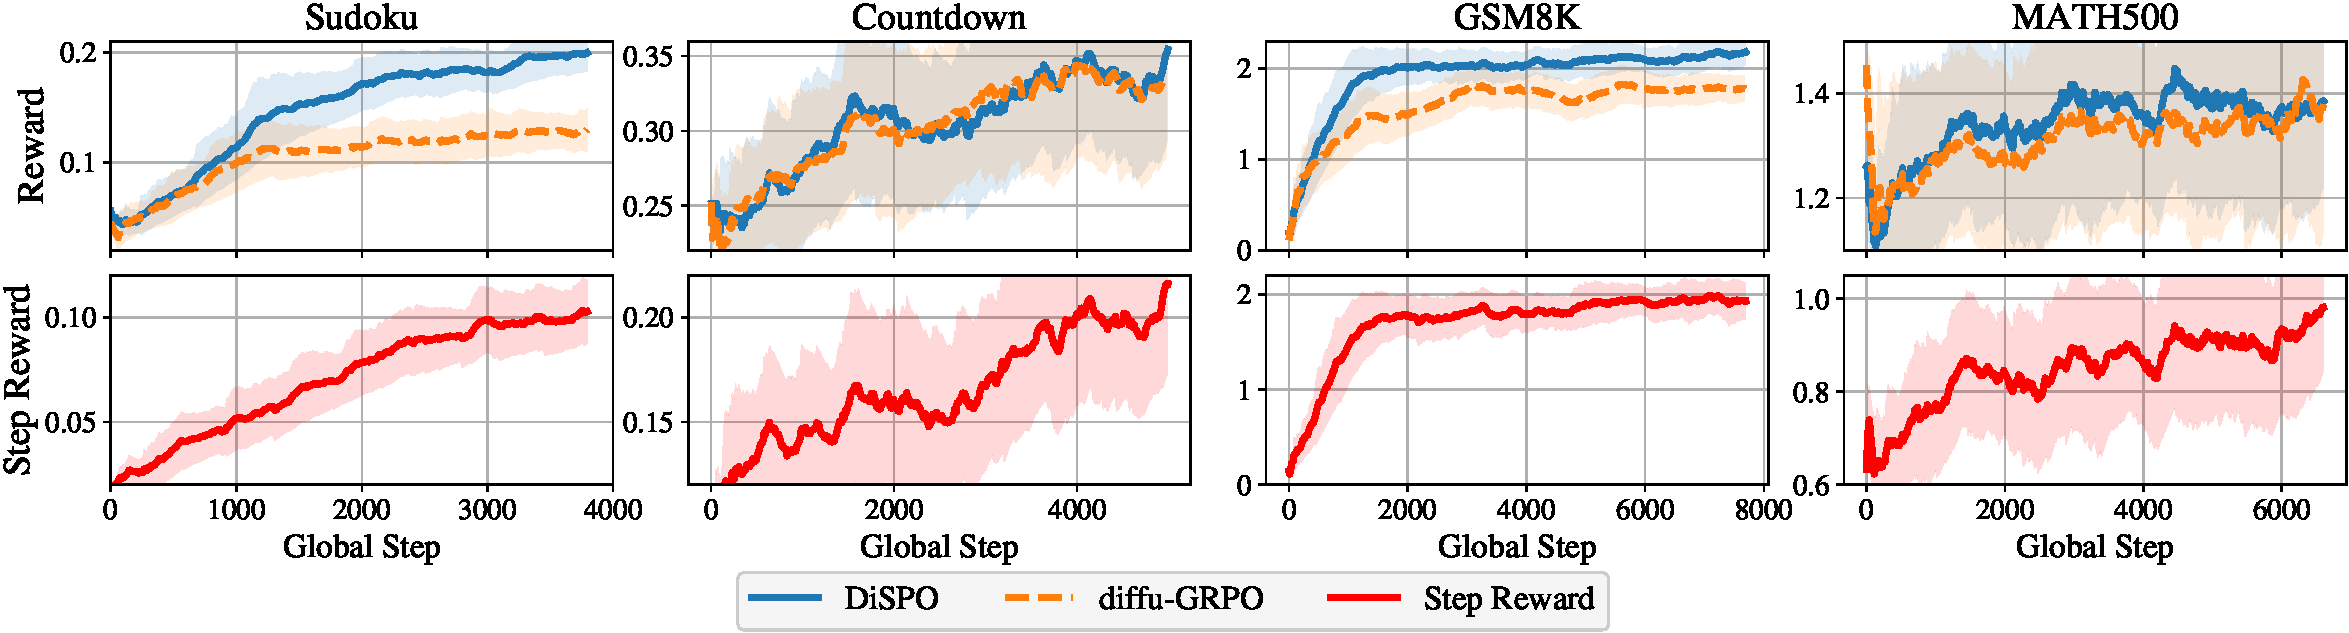
\includegraphics[width=0.9\textwidth]{reward_combined_8.pdf}
  \caption{\textbf{Reward curves.} Terminal reward curves (\emph{top}) and step reward curves (\emph{bottom}) on LLaDA-8B-Instruct during policy optimization. Across tasks, \method\ reaches higher terminal rewards earlier and maintains them over training. Step rewards exhibit relatively smaller magnitudes but follow trends as terminal rewards, indicating their role as a complementary training signal.}
  \label{fig:qualitative-2x2}
\end{figure*}



\section{Experiments}
\label{sec:experiments}
This section evaluates whether incorporating intermediate-state updates improves policy optimization for MDLMs.
Since \method\ naturally augments terminal-feedback optimization with a state-wise objective~(Algo.~\ref{alg:dispo}; Eq.~\ref{eq:app-mixed-grad-decomp}), 
we use the most direct baseline: diffu-GRPO~\citep{zhao2025d1}.
To isolate the effect of state-conditioned credit assignment, 
we match training budgets by fixing 
i) the number of full diffusion rollouts, 
ii) the sequence-level group size, 
and iii) the number of RL update steps;
\method\ resamples by reusing cached-logit within each rollout.


\subsection{Setup}
\label{sec:setup}

\textbf{Models.}
We evaluate LLaDA-8B-Instruct~\citep{nie2025largelanguagediffusionmodels} and a variant further fine-tuned on s1k~\citep{s1k}.
Across methods, we follow the identical fine-tuning and RL recipe of \citet{zhao2025d1} and keep the denoising schedule fixed. See Appendix~\ref{app:exp:setting} for more details.

\textbf{Benchmarks and metrics.}
Following \citet{zhao2025d1}, we report exact-match accuracy on benchmarks for math reasoning (GSM8K~\citep{gsm8k}; MATH500~\citep{lightman2023lets}) and symbolic planning (Sudoku; Countdown~\citep{zhao2025d1}).
See Appendix~\ref{app:exp:benchmark} for details.

\textbf{Optimization.}
For fair comparison, we match the baseline training setup across methods (including $N_{\text{gen}}{=}256$, denoising schedule, rollout budget, and the number of RL updates) and reuse the same terminal reward evaluator for both terminal and state-wise terms.
Unless stated otherwise, \method\ uses $Z{=}2$, samples one timestep per rollout from a \emph{late-biased} polynomial distribution (degree $k{=}4$), and sets $\alpha_{\text{step}}{=}0.1$; remaining hyperparameters are in Appendix~\ref{app:exp:setting}.


\textbf{Evaluation.}
We follow the protocol of diffu-GRPO~\citep{zhao2025d1}.
We evaluate at $N_{\text{gen}}\in\{128,256,512\}$ using zero-shot greedy decoding.
For diffusion decoding, we use $N_{\text{gen}}/2$ denoising steps with a block size of 32 tokens.
We provide more details in Appendix~\ref{app:exp:inference}.


\subsection{Main results}
\label{sec:main-results}
Table~\ref{tab:main-results} reports exact-match accuracy on four benchmarks for $N_{\text{gen}}\!\in\!\{128,256,512\}$.
At the default generation length ($N_{\text{gen}}{=}256$), \method\ outperforms terminal-feedback diffu-GRPO across all model--benchmark pairs, with gains largely persisting at other generation lengths, including Avg.

Importantly, these gains are obtained under matched rollout forward passes and parameter-update steps, using the same terminal reward evaluator for both terminal and state-wise updates.
This suggests the improvements come from finer-grained, state-wise credit assignment rather than extra rollouts or additional reward shaping.

To probe the underlying training dynamics, Fig.~\ref{fig:qualitative-2x2} plots both terminal rewards (\textit{top}) and step rewards (\textit{bottom}) on LLaDA-8B-Instruct.
\method\ reaches higher terminal rewards earlier and sustains them throughout training; while step rewards vary over a smaller range, they track the up and downs of terminal reward, consistent with a state-wise signal that aligns with terminal feedback along the trajectory.



\begin{figure}[t]
    \centering
    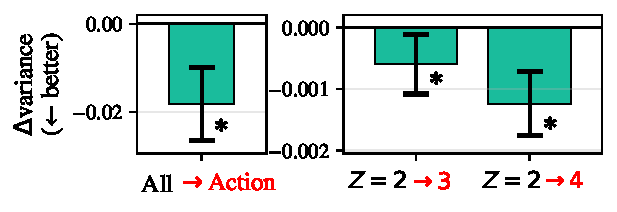
\includegraphics[width =0.95\linewidth]{pair_vs_action2_bar_split_swap.pdf}

\caption{\textbf{Variance reduction of the step-wise gradient estimator on Sudoku.}
    \textbf{\textit{Left}}: Updating only action tokens (vs.\ all tokens) reduces variance at $Z{=}2$ (Prop.~\ref{prop:var}).
    \textbf{\textit{Right}}: Increasing $Z$ from $Z{=}2$ reduces variance with action-only updates (Prop.~\ref{prop:compute}).
    Error bars show paired 95\% bootstrap CIs.}

  \label{fig:gradvar}
\end{figure}



\begin{table}[t]
\centering
\small
\caption{\textbf{Step-wise estimator design on Sudoku.}
Exact-match accuracy (\%) when varying gradient scope (Prop.~\ref{prop:var}) and the number of same-state drafts $Z$ (Prop.~\ref{prop:compute}).}
\begin{tabular}{l@{\,\,}lllll}
\toprule
\multicolumn{2}{l}{\textbf{Perspectives} ~$\backslash$~ $N_\text{gen}$} & {\textbf{128}} & {\textbf{256}} & {\textbf{512}} & {\textbf{Avg.}} \\
\midrule
\multirow{2}{*}{\rotatebox[origin=c]{90}{\textbf{\scriptsize{Grad.}}}}
& $\triangleright$ All tokens & {22.7} & {21.4} & {\textbf{20.6}} & {21.6} \\
& $\triangleright$ Action tokens only & \textbf{26.6}& \textbf{23.3} & 20.0 & \textbf{23.3} \\
\midrule
\multirow{3}{*}{\rotatebox[origin=c]{90}{\textbf{\scriptsize{\# Drafts}}}}
& $\triangleright$ $Z=2$ & {\textbf{26.6}} & {\textbf{23.3}} & {20.0} & {\textbf{23.3}} \\
& $\triangleright$ $Z=3$ & 25.1 & 22.8 & \textbf{21.0} & 23.0 \\
& $\triangleright$ $Z=4$ & \textbf{26.6} & 22.1 & 19.6 & 22.8 \\
\bottomrule
\end{tabular}
\label{tab:ablation-variance}
\end{table}



\subsection{Analysis: State-wise Estimator Design}
\label{sec:ablation-variance}
Propositions~\ref{prop:var} and~\ref{prop:compute} motivate two variance-reduction choices for intermediate-state policy optimization: (A) updating only actionable (newly filled) tokens and (B) averaging over $Z$ same-state drafts.
We evaluate both on 4$\times$4 Sudoku via lightweight, controlled comparisons of step-wise gradient variance and task performance.

\textbf{Empirical verification of gradient variance.}
To test the variance predictions, we measure the variance of the \emph{state-wise} gradient estimator.
At the last checkpoint for LLaDA-8B-Instruct in Sudoku, we repeatedly resample rollouts from the \emph{same set of states} and estimate the trace covariance of the resulting state-wise gradient estimates, $\mathrm{trCov}(\hat g)$.
Figure~\ref{fig:gradvar} shows that (\textit{left}) switching from all-token to actionable-token updates at $Z{=}2$ reduces $\mathrm{trCov}(\hat g)$, and (\textit{right}) increasing $Z$ under actionable-only updates reduces it, consistent with Propositions~\ref{prop:var} and~\ref{prop:compute} (Appendix~\ref{app:gradvar}).

\textbf{Impact on task performance.}
We then assess how these choices affect accuracy under the same training budget.
Table~\ref{tab:ablation-variance} (top) shows that updating all tokens underperforms the actionable-only, supporting alignment with the state--action decomposition.
Sweeping $Z\in\{2,3,4\}$ (bottom), we observe occasional gains at specific $N_{\text{gen}}$ but no monotonic improvement in average; we therefore use $Z{=}2$ by default.



\begin{table}[t]
\centering
\small
\caption{\textbf{Ablations of the optimization recipe on Sudoku}: timestep sampling, loss components, and step-loss intensity $\alpha_{\text{step}}$.}
\begin{tabular}{l@{\,\,}lllll}
\toprule
\multicolumn{2}{l}{\textbf{Perspectives} ~$\backslash$~ $N_\text{gen}$} & {\textbf{128}} & {\textbf{256}} & {\textbf{512}} & {\textbf{Avg.}} \\
\midrule
\multirow{3}{*}{\rotatebox[origin=c]{90}{\textbf{\scriptsize{Timestep}}}}
& $\triangleright$ Uniform & {25.1} & {23.0} & {17.5} & {21.9} \\
& $\triangleright$ Early-focused & {24.2} & {18.1} & {16.0} & {19.4} \\
& $\triangleright$ Late-focused & {\textbf{26.6}} & {\textbf{23.3}} & {\textbf{20.0}} & {\textbf{23.3}} \\
\midrule
\multirow{3}{*}{\rotatebox[origin=c]{90}{\textbf{\scriptsize{Loss}}}}
& $\triangleright$ $\mathcal{L}_{\text{term}}$ only & {18.4} & {12.9} & {11.0} & {14.1} \\
& $\triangleright$ $\mathcal{L}_{\text{step}}$ only & {24.9} & {18.4} & {17.7} & {20.3} \\
& $\triangleright$ Both & \textbf{26.6} & \textbf{23.3} & \textbf{20.0} & \textbf{23.3} \\
\midrule
\multirow{4}{*}{\rotatebox[origin=c]{90}{\textbf{\scriptsize{Intensity}}}}
& $\triangleright$ $\alpha_{\text{step}}=0.0$ & {18.4} & {12.9} & {11.0} & {14.1} \\
& $\triangleright$ $\alpha_{\text{step}}=0.1$ & {26.6} & {23.3} & {20.0} & {23.3} \\
& $\triangleright$ $\alpha_{\text{step}}=0.5$ & \textbf{34.7} & \textbf{30.2} & \textbf{29.4} & \textbf{31.4} \\
& $\triangleright$ $\alpha_{\text{step}}=0.9$ & {28.8} & {27.8} & {26.3} & {27.6} \\
\bottomrule
\end{tabular}
\label{tab:ablation}
\end{table}



\begin{figure}[b]
  \centering
  \begin{subfigure}[t]{0.12\textwidth}
    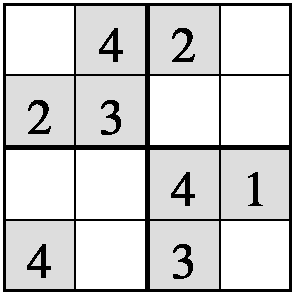
\includegraphics[width=\linewidth]{sudoku_input_big.pdf}
    \caption{Input}
  \end{subfigure}\hspace{2.4mm}
  \begin{subfigure}[t]{0.12\textwidth}
    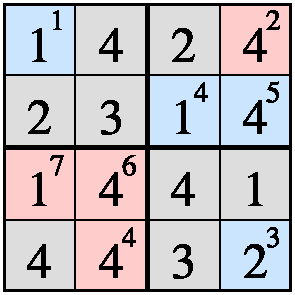
\includegraphics[width=\linewidth]{sudoku_diffu_grpo_big.pdf}
    \caption{diffu-GRPO}
  \end{subfigure}\hspace{2.4mm}
  \begin{subfigure}[t]{0.12\textwidth}
    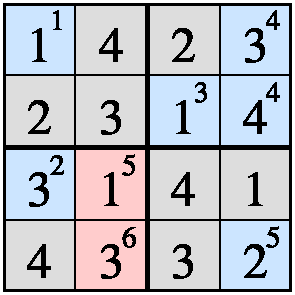
\includegraphics[width=\linewidth]{sudoku_dispo_big.pdf}
    \caption{DiSPO}
  \end{subfigure}
  \caption{\textbf{Example of error completion in Sudoku}. Red/blue indicate incorrect/correct fillings; superscripts denote the fill order. diffu-GRPO violates constraints earlier than \method.} 
  \label{fig:sudoku-case}
\end{figure}


\begin{figure}[t]
  \centering
  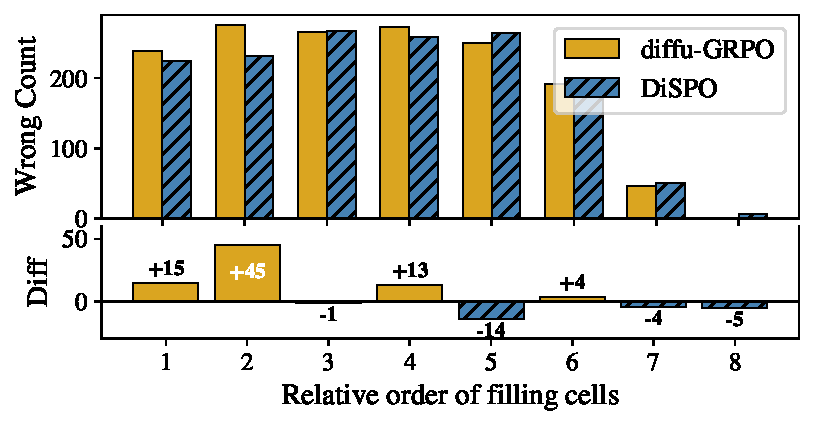
\includegraphics[width=0.9\linewidth]{rank_wrong_with_diff_tight_v2.pdf}
  \caption{\textbf{First-violation time on Sudoku.}
  The first-violation time is the earliest denoising step at which the filled cells violate Sudoku constraints.
  \method\ shifts violations to later steps than diffu-GRPO, indicating fewer premature commitments.}
  \label{fig:first-violation-hist}
\end{figure}


\subsection{Ablations: Optimization Recipe}
\label{sec:ablation}
We ablate three design choices for optimization: 
(i) which intermediate states to train on,
(ii) the optimization objective, 
and (iii) weight for the step-wise objective ($\alpha_{\text{step}}$).

\textbf{Timestep sampling.}
We compare uniform sampling to polynomial samplers ($k{=}4$) that bias draws toward late timesteps (near terminal states) or early timesteps (its mirrored variant).
Table~\ref{tab:ablation} (top) shows that late-biased sampling performs best, suggesting that very early masked states are too noisy for reliable credit assignment.

\textbf{Objectives.}
Table~\ref{tab:ablation} (middle) shows that $\mathcal{L}_{\text{step}}$ alone outperforms $\mathcal{L}_{\text{term}}$ alone, and combining them performs best, indicating complementary learning signals.

\textbf{Intermediate-state weight.}
Table~\ref{tab:ablation} (bottom) shows that, 
sweeping $\alpha_{\text{step}}\!\in\!\{0.1,0.5,0.9\}$, performance consistently stays above $\alpha_{\text{step}}{=}0$. 
However, gains are non-monotonic (best at $\alpha_{\text{step}}{=}0.5$), indicating its optimisation potential.




\subsection{Error Analysis: Early Commitments}
\label{sec:qual}
We analyze early-commitment errors using the final checkpoint of LLaD-8B-Instruct for Sudoku. We use $N_{\text{gen}}{=}128$; all other settings match the main experiments.

Figure~\ref{fig:sudoku-case} compares the same instance at the same denoising step: diffu-GRPO already violates constraints due to an early incorrect fill, whereas \method\ maintains a consistent partial assignment.
Figure~\ref{fig:first-violation-hist} corroborates this at scale---the first-violation time occurs later with \method.
These indicate that state-wise optimization reduces premature, hard-to-correct commitments during denoising.



\subsection{Compute Cost Breakdown}
\label{sec:exp:compute}

\textbf{Algorithmic overhead.}
Table~\ref{tab:compute-budget} shows per-prompt operation counts.
\method\ matches the dominant costs---diffusion-rollout forward passes ($KT$) and optimizer updates ($U$)---and adds only lightweight extras: reward evaluations for same-state branches and \emph{one-step} surrogate calls to compute step-wise log-probs at selected states.

\textbf{Wall-clock overhead and efficiency.}
Our current implementation is slower ($\sim$0.4$\times$ baseline throughput at $Z{=}2$ and $|\mathcal{S}|{=}K$), largely due to non-optimized repeated policy/surrogate calls and kernel/IO overhead; we discuss likely causes and optimizations in Appendix~\ref{app:wallclock}.
To account for this, Fig.~\ref{fig:wallclock} compares wall-clock-matched training curves: although \method\ starts slower, it catches up and surpasses the terminal-feedback baseline within the same time budget, indicating improved performance per unit time from better credit assignment rather than extra rollout/update compute.


\begin{table}[t]
\centering
\footnotesize
\caption{\textbf{Operation counts per prompt.}
$K$: \# rollouts, $T$: \# denoising steps/rollout, $\mathcal{S}$: set of selected states, $Z$: \# branches/state, $N_m$: \# monte-carlo prompt masks to estimate $\mathbb{E}_m[\cdot]$ in the surrogate, $U$: \# update steps.}
\label{tab:compute-budget}
\begin{tabular}{@{}l@{}cc@{}}
\toprule
\textbf{Compute items} & \textbf{w/o \method} & \textbf{w/ \method} \\
\midrule
Diffusion rollout forward passes & $KT$ & $KT$ \\
Optimizer update steps & $U$ & $U$ \\
One-step surrogate (terminal logps) & $2N_mK$ & $2N_mK$ \\
\midrule
Reward evaluations & $K$ & $K + \roundboxblue{$|\mathcal{S}|Z$}$ \\
One-step surrogate (step-wise logps) & $0$ & \roundboxblue{$2N_m|\mathcal{S}|$} \\
\bottomrule
\end{tabular}
\end{table}


\begin{figure}[t]
    \centering
    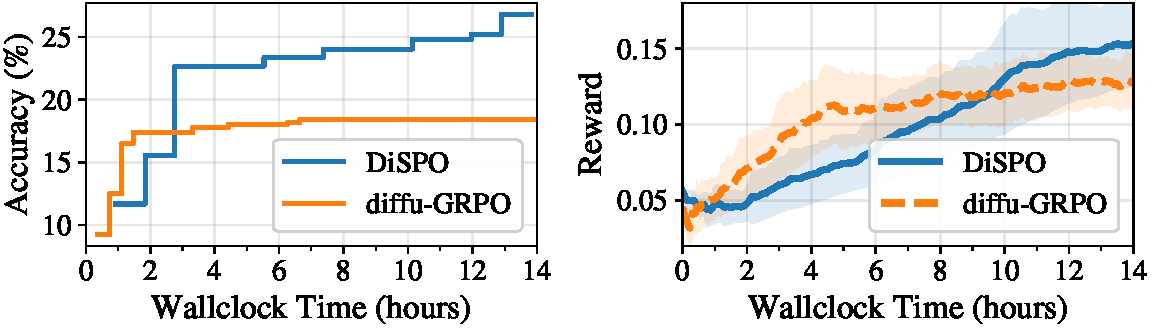
\includegraphics[width=\linewidth]{sudoku_combined_v2.pdf}
\caption{\textbf{Wall-clock-matched training curves on LLaDA-8B-Instruct for Sudoku.} Accuracy ($N_\mathrm{gen}{=}128$) and reward vs.\ training time. \method\ surpasses diffu-GRPO within the budget.}
    \label{fig:wallclock}
\end{figure}






\section{Related Work}
\label{sec:related} 

\textbf{Terminal-feedback policy optimization for MDLMs.}
Most RL fine-tuning methods for masked diffusion LMs use a scalar \emph{terminal} reward on the final completion and perform PPO/GRPO-style updates via surrogate likelihoods~\citep{zhao2025d1,tang2025wd1,cjgrpo,gdpo,spg,sepo,diffpo}. 
Our method differs by performing \emph{state-conditioned} comparisons: at a fixed intermediate state, we contrast alternative mask fillings (actions) rather than only learning from terminal rollouts.


\textbf{State-aware reward shaping.}
SAPO scores intermediate denoising states to build step-aware bonuses that \emph{shape the terminal signal}~\citep{sapo}, typically requiring \emph{additional multi-step rollouts}.
In contrast, \method\ directory optimizes intermediate-state actions without extra rollouts; a reference comparison is provided in Appendix~\ref{app:sapo}.


\textbf{Trajectory-level objectives.}
MDPO aligns with the denoising trajectory by comparing \emph{different rollouts} across steps and favoring trajectories whose intermediate predictions improve toward the terminal outcome~\citep{mdpo}.
In contrast, \method\ uses a different optimization unit: it fixes an intermediate state and compares alternative mask fillings.


\textbf{Surrogate likelihoods and gradient estimators.}
Complementary work improves surrogate likelihoods or policy-gradient estimators for diffusion LMs~\citep{spg,sepo,gdpo,d2}.
\method\ can directly incorporate improved surrogates/estimators while keeping the state-wise objective unchanged.




\section{Conclusion}\label{sec:conclusion}
We propose \method, a plug-in intermediate-state credit-assignment layer for policy optimization of masked diffusion language models, grounded in a policy-gradient formulation (\S~\ref{sec:method}).
This formulation induces step-wise and mixed objectives with principled policy-gradient estimators, and we analyze its variance reduction mechanisms (\S~\ref{sec:theory}).
Empirically, instantiating \method\ on top of terminal-feedback diffu-GRPO, we consistently improve accuracy across math and planning tasks under matched rollout forward passes and update steps using the same terminal reward (\S~\ref{sec:experiments}).

\textbf{Limitations and discussion.}
\method\ is a plug-in state-wise credit-assignment layer; future work includes pairing it with other terminal-feedback objectives (e.g., GDPO~\citep{gdpo}) and improved surrogate likelihood or gradient estimators (e.g., SPG~\citep{spg}).
We also use an unshaped terminal reward; studying complementarity with reward shaping (e.g., SAPO~\citep{sapo}) would clarify their interaction.



\clearpage
\section*{Impact Statement}
This paper presents work whose goal is to advance the field of Machine Learning by improving policy optimization for masked diffusion language models.
There are many potential societal consequences of improved language-model reasoning capabilities, including both beneficial applications and possible misuse; we do not believe our method introduces unique ethical concerns beyond those common to this line of research.

\section*{Acknowledgement}
These research results were obtained from the commissioned research (No.22501) by National Institute of Information and Communications Technology (NICT) , Japan.
This work was partially supported by JSPS KAKENHI Grant Number 25H01137 and JST K Program Japan Grant Number JPMJKP24C3.


\bibliography{example_paper}
\bibliographystyle{icml2026}

%%%%%%%%%%%%%%%%%%%%%%%%%%%%%%%%%%%%%%%%%%%%%%%%%%%%%%%%%%%%%%%%%%%%%%%%%%%%%%%
%%%%%%%%%%%%%%%%%%%%%%%%%%%%%%%%%%%%%%%%%%%%%%%%%%%%%%%%%%%%%%%%%%%%%%%%%%%%%%%
% APPENDIX
%%%%%%%%%%%%%%%%%%%%%%%%%%%%%%%%%%%%%%%%%%%%%%%%%%%%%%%%%%%%%%%%%%%%%%%%%%%%%%%
%%%%%%%%%%%%%%%%%%%%%%%%%%%%%%%%%%%%%%%%%%%%%%%%%%%%%%%%%%%%%%%%%%%%%%%%%%%%%%%
\newpage
\appendix
\onecolumn
\section{Proofs}\label{app:proofs}

\subsection{Proof of Theorem~\ref{thm:step-pg}}
\label{app:proof-step-pg}

We prove that the (unclipped) step-level loss yields a principled (scaled) policy-gradient estimator for the step-wise objective $J_t(\theta)$ when treating the surrogate $\tilde{\pi}_\theta$ as the policy.


\textbf{Setup.}
Fix a timestep index $t$. Recall the step-wise objective (Eq.~\ref{eq:Jt-def})
\[
  J_t(\theta)
  =
  \mathbb{E}_{q \sim \mathcal{D}}
  \mathbb{E}_{s_t \sim d_t(q)}
  \mathbb{E}_{a \sim \tilde{\pi}_\theta(\cdot \mid s_t)}
  \bigl[ R\bigl(q,\textsc{Fill}(x_t,a)\bigr) \bigr],
\]
where $s_t=(q,x_t)$ and $a$ fills the masked positions at $s_t$.
For brevity, define the terminal reward as a function of $(s_t,a)$:
\[
  \mathcal{R}(s_t,a) := R\bigl(q,\textsc{Fill}(x_t,a)\bigr).
\]

\textbf{Policy-gradient form of $\nabla_\theta J_t(\theta)$.}
Under Assumption~(i) of Theorem~\ref{thm:step-pg}, the state distribution
$d_t(q)$ is induced by the frozen behavior model $\theta_{\text{old}}$ and
is independent of $\theta$, so we may move the gradient through the outer
expectations:
\begin{align}
\nabla_\theta J_t(\theta)
&=
\mathbb{E}_{q \sim \mathcal{D}}
\mathbb{E}_{s_t \sim d_t(q)}
\left[
\nabla_\theta
\mathbb{E}_{a \sim \tilde{\pi}_\theta(\cdot \mid s_t)}
\bigl[\mathcal{R}(s_t,a)\bigr]
\right].
\label{eq:app-Jt-movegrad}
\end{align}
Under Assumption~(ii) (differentiable, normalized $\tilde{\pi}_\theta$), the
score-function identity gives
\[
\nabla_\theta
\mathbb{E}_{a \sim \tilde{\pi}_\theta(\cdot \mid s_t)}
\bigl[\mathcal{R}(s_t,a)\bigr]
=
\mathbb{E}_{a \sim \tilde{\pi}_\theta(\cdot \mid s_t)}
\bigl[\mathcal{R}(s_t,a)\,\nabla_\theta \log \tilde{\pi}_\theta(a \mid s_t)\bigr].
\]
Substituting into Eq.~\ref{eq:app-Jt-movegrad} yields
\begin{equation}
\nabla_\theta J_t(\theta)
=
\mathbb{E}_{q \sim \mathcal{D}}
\mathbb{E}_{s_t \sim d_t(q)}
\mathbb{E}_{a \sim \tilde{\pi}_\theta(\cdot \mid s_t)}
\bigl[\mathcal{R}(s_t,a)\,\nabla_\theta \log \tilde{\pi}_\theta(a \mid s_t)\bigr].
\label{eq:app-Jt-pg}
\end{equation}

\textbf{Expected gradient of the step-level loss.}
At a selected state $s_{k,t}$, DiSPO draws $Z$ branched action samples
$a_{k,t,1:Z}$ from the frozen behavior policy $\tilde{\pi}_{\theta_{\text{old}}}(\cdot\mid s_{k,t})$
and evaluates $\mathcal{R}(s_{k,t},a_{k,t,z})$ for each branch.
Ignoring clipping (as stated in the theorem), the per-state step loss is
\[
  \mathcal{L}_{\text{step}}^{(k,t)}(\theta)
  =
  -\frac{1}{Z}\sum_{z=1}^Z
  \rho_{k,t,z}(\theta)\,A_{k,t,z},
  \qquad
  \rho_{k,t,z}(\theta)
  :=
  \frac{\tilde{\pi}_\theta(a_{k,t,z}\mid s_{k,t})}{\tilde{\pi}_{\theta_{\text{old}}}(a_{k,t,z}\mid s_{k,t})},
\]
where $A_{k,t,z}$ is the group-relative advantage using the within-group mean baseline (Eq.~\ref{eq:group-adv}), i.e., $A_{k,t,z}=R_{k,t,z}-\bar R_{k,t}$ with $\bar R_{k,t}=\frac{1}{Z}\sum_{j=1}^Z R_{k,t,j}$.
Since $\tilde{\pi}_{\theta_{\text{old}}}$ is frozen, $\nabla_\theta \rho_{k,t,z}(\theta)
=
\rho_{k,t,z}(\theta)\,\nabla_\theta \log \tilde{\pi}_\theta(a_{k,t,z}\mid s_{k,t})$.
Therefore,
\begin{equation}
-\nabla_\theta \mathcal{L}_{\text{step}}^{(k,t)}(\theta)
=
\frac{1}{Z}\sum_{z=1}^Z
\rho_{k,t,z}(\theta)\,A_{k,t,z}\,\nabla_\theta \log \tilde{\pi}_\theta(a_{k,t,z}\mid s_{k,t}).
\label{eq:app-step-grad}
\end{equation}


Taking expectation over the branched samples $a_{k,t,1:Z}\sim \tilde{\pi}_{\theta_{\text{old}}}(\cdot\mid s_{k,t})$
and using importance weighting yields
\begin{align}
\mathbb{E}\bigl[-\nabla_\theta \mathcal{L}_{\text{step}}^{(k,t)}(\theta)\mid q,s_{k,t}\bigr]
&=
\mathbb{E}_{a_{1:Z} \sim \tilde{\pi}_\theta(\cdot\mid s_{k,t})}
\left[
\frac{1}{Z}\sum_{z=1}^Z (R_z-\bar R)\,\nabla_\theta \log \tilde{\pi}_\theta(a_z\mid s_{k,t})
\right],
\label{eq:app-step-exp1-new}
\end{align}
where $R_z=\mathcal{R}(s_{k,t},a_z)$ and $\bar R=\frac{1}{Z}\sum_{j=1}^Z R_j$.
Expanding the baseline term,
\[
\mathbb{E}\!\left[\frac{1}{Z}\sum_{z=1}^Z \bar R\,\nabla_\theta \log \tilde{\pi}_\theta(a_z\mid s_{k,t})\right]
=
\frac{1}{Z^2}\sum_{z=1}^Z\sum_{j=1}^Z
\mathbb{E}\!\left[R_j\,\nabla_\theta \log \tilde{\pi}_\theta(a_z\mid s_{k,t})\right].
\]
For $j\neq z$, $R_j$ is independent of $a_z$ and
$\mathbb{E}[\nabla_\theta \log \tilde{\pi}_\theta(a_z\mid s_{k,t})]=0$, so cross terms vanish.
Only the $j=z$ terms remain, yielding
\[
\mathbb{E}\!\left[\frac{1}{Z}\sum_{z=1}^Z \bar R\,\nabla_\theta \log \tilde{\pi}_\theta(a_z\mid s_{k,t})\right]
=
\frac{1}{Z}\,
\mathbb{E}_{a \sim \tilde{\pi}_\theta(\cdot\mid s_{k,t})}
\bigl[\mathcal{R}(s_{k,t},a)\,\nabla_\theta \log \tilde{\pi}_\theta(a\mid s_{k,t})\bigr].
\]
Therefore,
\[
\mathbb{E}\bigl[-\nabla_\theta \mathcal{L}_{\text{step}}^{(k,t)}(\theta)\mid q,s_{k,t}\bigr]
=
\frac{Z-1}{Z}\,
\mathbb{E}_{a \sim \tilde{\pi}_\theta(\cdot\mid s_{k,t})}
\bigl[\mathcal{R}(s_{k,t},a)\,\nabla_\theta \log \tilde{\pi}_\theta(a\mid s_{k,t})\bigr].
\]
Taking outer expectations over $q\sim\mathcal{D}$ and $s_{k,t}\sim d_t(q)$ yields
\[
\mathbb{E}\bigl[-\nabla_\theta \mathcal{L}_{\text{step}}^{(t)}(\theta)\bigr]
=
\frac{Z-1}{Z}\,\nabla_\theta J_t(\theta),
\]
which matches Theorem~\ref{thm:step-pg}. \qed


\textbf{Remark on the group baseline.}
If a leave-one-out baseline is used (independent of each branch action), the estimator is unbiased.
With the within-group mean baseline in Eq.~\ref{eq:group-adv} used in our implementation, the expected gradient is scaled by the constant factor $(Z-1)/Z$, which can be absorbed into $\alpha_{\text{step}}$ or the learning rate.



\subsection{Proof of Theorem~\ref{thm:mixed}}
\label{app:proof-mixed}

We prove that the expected gradient of the combined loss equals the gradient of the mixed objective.
Throughout, we treat the masked-token surrogate $\tilde{\pi}_\theta$ as the policy being optimized and work in the unclipped setting stated in \S\ref{sec:theory-mixed}.

\textbf{Recall the mixed objective and combined loss.}
Let $c_Z := (Z-1)/Z$ denote the constant scaling induced by the within-group mean baseline in the step-wise estimator.
The mixed objective (Eq.~\ref{eq:Jmix-def}) is
\[
  J_{\text{mix}}(\theta)
  =
  \alpha_{\text{step}}\,c_Z\sum_t \omega(t)\,J_t(\theta)
  +
  \alpha_{\text{term}}\,J_{\text{seq}}(\theta),
\]
where $J_t(\theta)$ is the step-wise objective (Eq.~\ref{eq:Jt-def}) and $J_{\text{seq}}(\theta)$ is the terminal surrogate objective (Eq.~\ref{eq:Jseq-def}).
The combined training loss is
\[
  \mathcal{L}(\theta)
  =
  \alpha_{\text{step}}\,\mathcal{L}_{\text{step}}(\theta)
  +
  \alpha_{\text{term}}\,\mathcal{L}_{\text{term}}(\theta).
\]
By linearity of differentiation,
\begin{equation}
  \nabla_\theta J_{\text{mix}}(\theta)
  =
  \alpha_{\text{step}}\,c_Z\sum_t \omega(t)\,\nabla_\theta J_t(\theta)
  +
  \alpha_{\text{term}}\,\nabla_\theta J_{\text{seq}}(\theta).
  \label{eq:app-mixed-grad-decomp}
\end{equation}
It therefore suffices to show that
\(
\mathbb{E}\!\left[-\nabla_\theta \mathcal{L}_{\text{step}}(\theta)\right]
=
c_Z\sum_t \omega(t)\,\nabla_\theta J_t(\theta)
\)
and
\(
\mathbb{E}\!\left[-\nabla_\theta \mathcal{L}_{\text{term}}(\theta)\right]
=
\nabla_\theta J_{\text{seq}}(\theta).
\)

\textbf{Step term.}
Recall that $\mathcal{L}_{\text{step}}(\theta)$ is computed by selecting timesteps according to $\omega(t)$ and applying the per-state step loss $\mathcal{L}_{\text{step}}^{(k,t)}(\theta)$ (Eq.~\ref{eq:inter-loss-method}) on the corresponding intermediate state(s).
Condition on a particular timestep $t$ being selected.
Under the assumptions of Theorem~\ref{thm:step-pg}, we have
\[
  \mathbb{E}\!\left[-\nabla_\theta \mathcal{L}_{\text{step}}(\theta)\,\middle|\, t\right]
  =
  c_Z\,\nabla_\theta J_t(\theta),
\]
where the expectation is over $q\sim\mathcal{D}$, $s_t\sim d_t(q)$, and the branched action samples at that state.
Taking expectation over $t\sim\omega(t)$ yields
\begin{equation}
\mathbb{E}\!\left[-\nabla_\theta \mathcal{L}_{\text{step}}(\theta)\right]
  =
  c_Z\sum_t \omega(t)\,\nabla_\theta J_t(\theta).
  \label{eq:app-step-term}
\end{equation}

\textbf{Terminal term.}
By definition,
\[
  J_{\text{seq}}(\theta)
  =
  \mathbb{E}_{q\sim\mathcal{D}}
  \mathbb{E}_{o\sim\tilde{\pi}_\theta(\cdot\mid q)}
  \bigl[R(q,o)\bigr].
\]
A standard score-function (REINFORCE) argument gives
\[
  \nabla_\theta J_{\text{seq}}(\theta)
  =
  \mathbb{E}_{q,o\sim\tilde{\pi}_\theta}
  \bigl[
    R(q,o)\,\nabla_\theta \log \tilde{\pi}_\theta(o\mid q)
  \bigr],
\]
and subtracting any baseline that depends on $q$ but not on $o$ preserves unbiasedness.
The terminal GRPO loss $\mathcal{L}_{\text{term}}(\theta)$ is precisely the corresponding baseline-centered (and, in practice, importance-weighted) estimator; in the unclipped setting,
\begin{equation}
  \mathbb{E}\!\left[-\nabla_\theta \mathcal{L}_{\text{term}}(\theta)\right]
  =
  \nabla_\theta J_{\text{seq}}(\theta),
  \label{eq:app-term-term}
\end{equation}
which is the standard PPO/GRPO identity (see, e.g.,~\citet{shao2024deepseekmath}).

\textbf{Combine the terms.}
Combining Eq.~\ref{eq:app-step-term} and Eq.~\ref{eq:app-term-term} and using linearity of expectation,
\[
\mathbb{E}\!\left[-\nabla_\theta \mathcal{L}(\theta)\right]
=
\alpha_{\text{step}}\,c_Z \sum_t \omega(t)\,\nabla_\theta J_t(\theta)
+
\alpha_{\text{term}}\,\nabla_\theta J_{\text{seq}}(\theta)
=
\nabla_\theta J_{\text{mix}}(\theta),
\]
where the last equality follows from Eq.~\ref{eq:app-mixed-grad-decomp} with the definition of $J_{\text{mix}}(\theta)$ above.
This proves Theorem~\ref{thm:mixed}. \qed


\textbf{Remark (KL-regularized case).}
If the main text includes a KL penalty, the same argument applies after adding the term
$-\lambda\,\mathbb{E}_{q}[\mathrm{KL}(\tilde{\pi}_\theta(\cdot\mid q)\,\|\,\tilde{\pi}_{\text{ref}}(\cdot\mid q))]$
to $J_{\text{mix}}(\theta)$ and the corresponding penalty $\lambda\,\mathcal{L}_{\text{KL}}(\theta)$ to $\mathcal{L}(\theta)$; differentiation under the expectation yields the additional gradient term.











\subsection{Proof of Proposition~\ref{prop:var}}
\label{app:proof-partial}

We prove the variance reduction claim for the token-local (action-only) estimator under the stated independence assumptions.

\textbf{Setup.}
Fix a diffusion state $s=(q,x)$ of length $L$ with masked set $M\subseteq[L]$ of size $m=|M|$.
Let $R$ denote the (scalar) terminal reward associated with the filled candidate, and define per-position score terms
\[
g_i \;:=\; \nabla_\theta \log \tilde{\pi}_\theta(a_i \mid s,i),
\]
where $a_i$ is the token sampled at position $i$ (for $i\in M$) and $\tilde{\pi}_\theta(\cdot\mid s,i)$ is the one-step surrogate distribution at position $i$.
Consider the two estimators (as in \S\ref{sec:theory-var})
\[
\hat g_{\text{full}} \;=\; \sum_{i=1}^L g_i\,R,
\qquad
\hat g_{\text{sub}} \;=\; \sum_{i\in M} g_i\,R.
\]

\textbf{Variance calculation.}
Under the assumptions of Proposition~\ref{prop:var}, $\{g_i\}_{i=1}^L$ are independent, zero-mean with $\mathrm{Var}[g_i]=\sigma^2$, and $R$ is independent of all $g_i$ with $\mathbb{E}[R^2]<\infty$.
First, independence across positions implies
\[
\mathrm{Var}\!\left[\sum_{i\in S} g_i R\right]
=
\sum_{i\in S} \mathrm{Var}[g_i R]
\quad\text{for any index set } S\subseteq[L].
\]
Second, since $g_i$ is independent of $R$ and $\mathbb{E}[g_i]=0$,
\[
\mathrm{Var}[g_i R]
=
\mathbb{E}[g_i^2 R^2] - (\mathbb{E}[g_i R])^2
=
\mathbb{E}[g_i^2]\mathbb{E}[R^2]
=
\sigma^2\,\mathbb{E}[R^2].
\]
Therefore,
\[
\mathrm{Var}[\hat g_{\text{full}}]
=
\sum_{i=1}^L \sigma^2\mathbb{E}[R^2]
=
L\,\sigma^2\mathbb{E}[R^2],
\qquad
\mathrm{Var}[\hat g_{\text{sub}}]
=
\sum_{i\in M} \sigma^2\mathbb{E}[R^2]
=
m\,\sigma^2\mathbb{E}[R^2].
\]
Taking the ratio yields
\[
\mathrm{Var}[\hat g_{\text{sub}}]
=
\frac{m}{L}\,\mathrm{Var}[\hat g_{\text{full}}],
\]
which implies the stated inequality in Proposition~\ref{prop:var} since $m\le L$.
\qed

\textbf{Remark (vector-valued gradients).}
If each $g_i$ is vector-valued, the same argument applies coordinate-wise.
Equivalently, writing $\mathrm{tr}\,\mathrm{Cov}[\cdot]$ for the trace of the covariance matrix, independence implies
$\mathrm{tr}\,\mathrm{Cov}[\hat g_{\text{sub}}] = \frac{m}{L}\,\mathrm{tr}\,\mathrm{Cov}[\hat g_{\text{full}}]$
under the same assumptions.




\subsection{Proof of Proposition~\ref{prop:compute}}
\label{app:proof-compute}

We prove the $O(1/Z)$ variance reduction from averaging $Z$ (approximately) independent branches at a fixed state.

\textbf{Setup.}
Fix a state $s$ and draw i.i.d.\ actions $a_1,\dots,a_Z \sim \tilde{\pi}_\theta(\cdot\mid s)$ with associated rewards $R_z$.
Let $b(s)$ be any baseline independent of each sampled action $a_z$, and define the per-branch contribution
\[
  \hat g_z \;:=\; (R_z-b(s))\,\nabla_\theta \log \tilde{\pi}_\theta(a_z\mid s).
\]
Define the averaged estimator
\[
  \hat g \;:=\; \frac{1}{Z}\sum_{z=1}^Z \hat g_z,
\]
and assume $\hat g_z$ have finite variance.

\textbf{Variance of an average.}
For the scalar case, independence gives
\[
\mathrm{Var}[\hat g]
=
\mathrm{Var}\!\left[\frac{1}{Z}\sum_{z=1}^Z \hat g_z\right]
=
\frac{1}{Z^2}\sum_{z=1}^Z \mathrm{Var}[\hat g_z]
=
\frac{1}{Z}\,\mathrm{Var}[\hat g_z],
\]
where $\mathrm{Var}[\hat g_z]$ is the same for all $z$ since $\{\hat g_z\}_{z=1}^Z$ are i.i.d.
Thus $\mathrm{Var}[\hat g]=O(1/Z)$.


For the vector-valued case, the same argument holds for covariance matrices. Under independence,
\[
\mathrm{Cov}[\hat g]
=
\mathrm{Cov}\!\left[\frac{1}{Z}\sum_{z=1}^Z \hat g_z\right]
=
\frac{1}{Z^2}\sum_{z=1}^Z \mathrm{Cov}[\hat g_z]
=
\frac{1}{Z}\,\mathrm{Cov}[\hat g_z],
\]
where the last equality uses that $\{\hat g_z\}_{z=1}^Z$ are i.i.d.\ and hence have identical covariance.
Therefore $\mathrm{tr}\,\mathrm{Cov}[\hat g] = \frac{1}{Z}\,\mathrm{tr}\,\mathrm{Cov}[\hat g_z] = O(1/Z)$.
\qed


\textbf{Remark (group-relative baseline used in practice).}
Our implementation uses the within-group mean baseline (Eq.~\ref{eq:group-adv}), which introduces dependence across branches.
Proposition~\ref{prop:compute} formalizes the standard $1/Z$ reduction for action-independent baselines; empirically, increasing $Z$ reduces variance in our setting as well (\S~\ref{sec:experiments}).














\appendix
\section{Experimental Details}
\label{app:exp}

This appendix provides additional details on benchmarks, reward functions, and training/implementation settings used in our experiments. We follow the d1/diffu-GRPO recipe wherever applicable~\citep{zhao2025d1}; in particular, our SFT procedure and programmatic reward evaluators are reused from d1. Exact run-specific hyperparameters (including optimizer schedules, seeds, and infrastructure settings) are recorded in the configuration files of our code scheduled for release.

\subsection{Benchmarks, Evaluation Protocol, and Reward Functions}
\label{app:exp:benchmark}

We evaluate on four reasoning benchmarks following \citet{zhao2025d1}. 
For each task, we report exact-match accuracy and use a programmatic verifier to compute a scalar reward $R(q,o)$ from the model completion $o$ given prompt $q$. 
Unless stated otherwise, rewards are binary ($1$ for a valid correct solution and $0$ otherwise), and \method\ applies the \emph{same} terminal reward function for both the sequence-level and state-wise objectives, i.e., \emph{non-reward shaping on terminal rewards and non-custom engineering for step-wise rewards}.
For fully fair comparison, implementations for the reward functions are reused from diffu-GRPO~\citep{zhao2025d1} without modification i.e., \url{https://github.com/dllm-reasoning/d1}.

\textbf{GSM8K.}
GSM8K~\citep{gsm8k} is a grade-school math word-problem benchmark.
It uses exact match on the final numeric answer after applying the same answer-extraction and normalization rules.
We use the training data publicly available \url{https://huggingface.co/datasets/openai/gsm8k}.
\emph{Reward} is computed by considering multiple axes, i.e., format reward (max. $1.625$) and correctness reward (max. $2.0$).

\textbf{MATH500.}
MATH500~\citep{lightman2023lets} is a subset of MATH focusing on competition-level problems.
\emph{Reward} is computed by considering the two axes, i.e., format reward (max $1.0$) and correctness reward (max $2.0$)

\textbf{Sudoku.}
4$\times$4 Sudoku tasks is synthetic benchmark for planning.
We use the training data publicly available \url{https://github.com/Black-Phoenix/4x4-Sudoku-Dataset}.
As for the evaluation data, we use the synthetically created problem set by using specific implementation \url{https://www.ocf.berkeley.edu/~arel/sudoku/main.html}.
Reward is the fraction of empty cells filled correctly.

\textbf{Countdown.}
Countdown is an arithmetic-planning benchmark, whose training data publicly available \url{https://huggingface.co/datasets/Jiayi-Pan/Countdown-Tasks-3to4}.
\emph{Evaluation} parses the output into an arithmetic expression, verifies that it uses the provided numbers under the task rules, and checks that the expression evaluates exactly to the target value.
\emph{Reward} is computed by considering the two axes, i.e., nearly-correct answers obtain $0.1$ and the perfect answers gain $1.0$.

\subsection{Inference Details}
\label{app:exp:inference}
For inference, we use semi-autoregressive decoding with 32-token blocks~\cite{arriolablock}, unmasking the 2 highest-confidence tokens per step within each block.
We evaluate at $N_{\text{gen}}\in\{128,256,512\}$ using zero-shot prompting and greedy decoding.


\subsection{Training and Implementation Details}
\label{app:exp:setting}

\textbf{Model variants and SFT.}
We evaluate two model variants:
(1) LLaDA-8B-Instruct~\citep{nie2025largelanguagediffusionmodels}, and
(2) its variant additionally fine-tuned on the s1k dataset~\citep{s1k}.
Across algorithms, we use the \emph{same} SFT recipe for each model variant (data, schedule, and hyperparameters), reusing the d1 implementation where applicable; \url{https://github.com/dllm-reasoning/d1}.
We keep the architecture, tokenizer, and denoising schedule fixed throughout.
Furthermore, to isolate the effect of state-wise updates, we match compute-relevant quantities across methods, including: the number of RL update steps (3800/5000/7700/6600 steps for Sudoku/Countdown/GSM8K/MATH500, respectively).
These are often task-dependent. Please refer to their experimental configuration.

\textbf{DiSPO-specific settings.}
Unless stated otherwise, DiSPO uses a conservative default settings.
Concretely, we set branch size $Z{=}2$ completion candidates per selected intermediate state with
a timestep-sampling distribution $q(t)$ for selecting intermediate time steps (\S~\ref{sec:experiments}), with polynomial exponent $k{=}4$, and loss weights $\alpha_{\text{step}}{=}0.1$ and $\alpha_{\text{term}}{=}1$.
We additionally specify the number of selected timesteps per trajectory $|T_{\text{sub}}|{=}1$ for light-weight evaluation. 

\textbf{Optimization.}
Following \citet{zhao2025d1},
we use LoRA with a rank $r=128$ and scaling factor $\alpha = 64$, and AdamW optimizer~\cite{}.
We basically set hyperparameters as follows: $\beta_1=0.9, \beta_2=0.99$, weight decay $0.1$, learning rate $5 \times 10^{-6}$, gradient clipping $0.2$. 
We train on $4$ NVIDIA H100-94G GPUs with batch size 6 per GPU, gradient accumulation steps of 4, and sequence length of 256 tokens. 


\section{Empirical Measurement of Step-level Gradient Variance}
\label{app:gradvar}

We detail the protocol used to produce Fig.~\ref{fig:gradvar}, which measures the variance of the step-level gradient estimator via repeated same-state branching.

\textbf{Quantity measured.}
Fix an intermediate diffusion state $s=(q,x)$ and draft size $Z$.
Let $\mathcal{L}_{\text{step}}(s;\theta)$ denote the \emph{unclipped} per-state step loss obtained by instantiating Eq.~\ref{eq:inter-loss-method} at state $s$ with $Z$ same-state branches, using the state-wise surrogate log-probability (Eq.~\ref{eq:subset-logprob-method}) and group advantages (Eq.~\ref{eq:group-adv}).
We define the step-level gradient estimator as the update direction
\[
\hat g_{\text{step}}(s)\;:=\;-\nabla_\theta \mathcal{L}_{\text{step}}(s;\theta)\in\mathbb{R}^d,
\]
We summarize the variance of this random vector by the trace covariance
\[
\mathrm{trCov}\bigl(\hat g_{\text{step}}(s)\bigr)
:=\mathrm{tr}\!\left(\mathrm{Cov}\bigl[\hat g_{\text{step}}(s)\bigr]\right)
=\mathbb{E}\!\left[\|\hat g_{\text{step}}(s)\|^2\right]-\left\|\mathbb{E}\!\left[\hat g_{\text{step}}(s)\right]\right\|^2.
\]
Empirically, for each fixed state $s$ we repeat same-state branching $R$ times to obtain $\{\hat g^{(r)}_{\text{step}}(s)\}_{r=1}^R$ and estimate
\[
\widehat{\mathrm{trCov}}\bigl(\hat g_{\text{step}}(s)\bigr)
=
\frac{1}{R-1}\sum_{r=1}^R \left\|\hat g^{(r)}_{\text{step}}(s)-\bar g_{\text{step}}(s)\right\|^2,
\qquad
\bar g_{\text{step}}(s)=\frac{1}{R}\sum_{r=1}^R \hat g^{(r)}_{\text{step}}(s).
\]



\textbf{Task, checkpoint, and state collection.}
We run this diagnostic on 4$\times$4 Sudoku for efficiency and use a fixed model checkpoint from DiSPO training (LLaDA optimized with DiSPO; step-3800).
We collect intermediate states from 64 prompts and sample 8 states per prompt, yielding 512 candidate states.

\textbf{State filtering and paired aggregation.}
To ensure a fair comparison across different conditions (e.g., different $Z$ and action-only vs full-token updates), we fix the same state set for all conditions and retain only non-degenerate states;
at the state (i) at least one actionable token contributes to the step loss (denominator $>0$), and
(ii) among the $R$ repeated branchings, at least one trial yields an advantage $>0$.
After filtering, we aggregate $\widehat{\mathrm{trCov}}(\hat g_{\text{step}}(s))$ over 276 states.

\textbf{Compared settings.}
$Z=2$ with action-only updates is the default setting used in our main experiments~(Table~\ref{tab:main-results}); 
Including that, for the $Z$ ablation, we test $Z\in\{2,3,4\}$; for the update-target ablation, we test the \emph{full-tokens} and \emph{action-only} variants.
Bars in Fig.~\ref{fig:gradvar} show the difference in gradient variance from the default ($Z=2$, action-only), with error bars indicating paired 95\% bootstrap CIs over states.






\section{Reference Comparison with Step-Aware Terminal Reward Shaping}\label{app:sapo}

\textbf{Difference in objectives.}
SAPO~\citep{sapo} and \method\ both leverage intermediate diffusion states, but they do so for different purposes.
SAPO scores intermediate states to \emph{shape the terminal rewards}, whereas \method\ directly optimizes \emph{intermediate-state actions}---the mask fillings sampled at a fixed partially-masked state---by comparing same-state counterfactual fillings under the unchanged terminal reward.
Hence, the two approaches are best viewed as complementary.

\textbf{Difference in compute.}
This difference in design also leads to substantially different compute profiles.
As summarized in Table~\ref{tab:compute-budget-sapo}, \method\ adds overhead mainly through extra reward evaluations for same-state branches and one-step surrogate evaluations for step-wise log-probabilities, while matching diffusion-rollout forward passes and update steps.
In contrast, SAPO typically incurs additional \emph{multi-step continuation rollouts} from intermediate states to estimate shaping terms, which increases the dominant cost---diffusion-rollout forward passes---often by a large margin.
Therefore, SAPO is not only complementary in approach, but can also be considerably more expensive in required rollout compute.


\begin{table}[h]
\centering
\caption{\textbf{Operation counts per prompt including SAPO.}
$K$: \# rollouts, $T$: \# denoising steps/rollout, $\mathcal{S}$: selected states (DiSPO), $Z$: \# branches/state,
$N_m$: \# MC prompt masks for $\mathbb{E}_m[\cdot]$, $U$: \# update steps.
For SAPO, $\mathcal{S}_{\mathrm{sapo}}$ is the set of intermediate states used for step-aware reward estimation,
$N_{\mathrm{sapo}}$ is the \# continuation rollouts per selected state, and $\bar T_{\mathrm{rem}}$ is the average remaining denoising steps.}
\label{tab:compute-budget-sapo}
\begin{tabular}{lccc}
\toprule
\textbf{Compute items} & \textbf{w/o \method} & \textbf{w/ \method} & \textbf{w/ SAPO} \\
\midrule
Diffusion rollout forward passes
& $KT$
& $KT$
& $KT + \roundboxorange{$N_{\mathrm{sapo}}|\mathcal{S}_{\mathrm{sapo}}|\bar T_{\mathrm{rem}}$}$ \\
Optimizer update steps
& $U$ & $U$ & $U$ \\
One-step surrogate (terminal logps)
& $2N_mK$ & $2N_mK$ & $2N_mK$ \\
\midrule
Reward evaluations
& $K$
& $K + \roundboxblue{$|\mathcal{S}|Z$}$
& $K + \roundboxorange{$N_{\mathrm{sapo}}|\mathcal{S}_{\mathrm{sapo}}|$}$ \\
One-step surrogate (step-wise logps)
& $0$
& \roundboxblue{$2N_m|\mathcal{S}|$}
& $0$ \\
\bottomrule
\end{tabular}
\end{table}




\textbf{Reference comparison in benchmarks.}
Despite the \emph{mismatch} in objectives and compute, SAPO is a representative step-aware method, so we include a \emph{reference} comparison to contextualize \method.
\textbf{\emph{This comparison should be interpreted with caution}}: the methods optimize different training signals (shaped vs.\ unshaped terminal rewards) and can require very different rollout compute (Table~\ref{tab:compute-budget-sapo}), so the evaluation is not an apples-to-apples matched-budget study.
To keep this reference study lightweight,
we report results on two representative benchmarks from our main suite: Sudoku (planning) and MATH500 (math), sweeping $\alpha_{\text{step}}\in\{0.1,0.5,0.9\}$.
Table~\ref{tab:sapo-sweep} reports that,
in 11/12 settings, \method\ outperforms SAPO, despite using substantially less rollout compute.


\begin{table*}[h]
\centering
\caption{\textbf{Reference comparison to SAPO.}
Exact-match accuracy (\%) on a planning task (Sudoku) and a math task (MATH500) at $N_{\text{gen}}\in\{128,256,512\}$.
\method\ is shown with a sweep of the step-loss weight $\alpha_{\text{step}}$, while SAPO uses its intermediate-state shaping signal.
This comparison is provided for context only (the methods optimize different intermediate-state signals and can differ in rollout compute; see Table~\ref{tab:compute-budget-sapo}).}
\label{tab:sapo-sweep}
\begin{tabular}{lr@{\,\,\,\,\,}r@{\,\,\,\,\,}r@{\,\,\,\,\,}rr@{\,\,\,\,\,}r@{\,\,\,\,\,}r@{\,\,\,\,\,}r}
\toprule
& \multicolumn{4}{c}{\textbf{Sudoku}} & \multicolumn{4}{c}{\textbf{MATH500}} \\
\cmidrule(lr){2-5}\cmidrule(lr){6-9}
\textbf{Methods} ~$\backslash$~ \textbf{$N_\text{gen}$} & \textbf{128} & \textbf{256} & \textbf{512} & \textbf{Avg.} & \textbf{128} & \textbf{256} & \textbf{512} & \textbf{Avg.} \\
\midrule
LLaDA-8B-Instruct & 11.7 & 6.7 & 5.5 & 8.0 & 26.0 & 32.4 & 36.2 & 31.5 \\
\quad $\triangleright$ diffu-GRPO & 18.4 & 12.9 & 11.0 & 14.1 & 33.2 & 37.2 & 39.2 & 36.5 \\
\rowcolor{gray!10}
\quad $\triangleright$ \method\ ($\alpha_{\text{step}}=0.1$) & 26.6 & 23.3 & 20.0 & 23.3 & \textbf{34.0} & {39.2} & \textbf{40.2} & \textbf{37.8} \\
\rowcolor{gray!10}
\quad $\triangleright$ \method\ ($\alpha_{\text{step}}=0.5$) & \textbf{34.7} & \textbf{30.2} & \textbf{29.4} & \textbf{31.4} & 33.2 & 38.4 & \textbf{40.2} & 37.3 \\
\rowcolor{gray!12}
\quad $\triangleright$ \method\ ($\alpha_{\text{step}}=0.9$) & 28.8 & 27.8 & 26.3 & 27.6 & 31.2 & 39.0 & 40.0 & 36.7 \\
\midrule
SAPO~\citep{sapo} & 22.4 & 20.3 & 16.1 & 19.6 & 32.0 & \textbf{40.0} & 38.4 & 36.8 \\
\bottomrule
\end{tabular}
\end{table*}


\textbf{Takeaway.}
These results suggest that, among ways to leverage intermediate diffusion states, \emph{directly optimizing intermediate mask-filling actions} can be a particularly effective alternative to using intermediate-state scores only for reward shaping, achieving competitive performance \emph{at a fraction of the rollout compute}.
At the same time, since SAPO and \method\ act on different axes (reward shaping vs.\ action-level optimization), they are potentially complementary; we leave a careful study of joint training recipes to future work.



\section{Discussion on the Wall-clock Overhead}
\label{app:wallclock}

\textbf{Observed overhead.}
In our current implementation, \method\ runs at lower throughput than the terminal-feedback baseline (reported in \S\ref{sec:exp:compute}) even at modest settings (e.g., $Z{=}2$).
This slowdown reflects engineering overhead rather than additional rollout/update compute, since the dominant algorithmic costs ($KT$ rollout forward passes and $U$ updates) are matched.

\textbf{Likely causes.}
The main contributors are repeated, non-amortized calls: (i) evaluating multiple same-state branches and (ii) computing step-wise log-probs via one-step surrogate calls at selected states.
When executed largely sequentially, these introduce frequent kernel launches, synchronization points, and host-side overhead that can dominate wall-clock time despite modest extra FLOPs.

\textbf{Optimization opportunities.}
These costs are not intrinsic to the method and should be reducible by (1) batching same-state branches (amortizing policy/surrogate/reward calls over $Z$), (2) caching state representations for step-wise terms, and (3) reducing kernel/IO overhead (e.g., call fusion / compilation and fewer synchronization points).
We therefore, as a reference, additionally reported wall-clock-matched curves (Fig.~\ref{fig:wallclock}) to ensure the performance gains (rewards and accuracy) are robust to current implementation overheads.



%%%%%%%%%%%%%%%%%%%%%%%%%%%%%%%%%%%%%%%%%%%%%%%%%%%%%%%%%%%%%%%%%%%%%%%%%%%%%%%
%%%%%%%%%%%%%%%%%%%%%%%%%%%%%%%%%%%%%%%%%%%%%%%%%%%%%%%%%%%%%%%%%%%%%%%%%%%%%%%

\end{document}

